\newpage
\section{実験}
\label{sec:method2}


\subsection{ロボットの構成}
使用するロボットには,外界のセンシング機能と不整地に対する一定の走破性能を持ったハードウェアがそれぞれ要求される.そこで使用するロボットには,図\ref{fig:fig}のような径の大きな2つのタイヤと2つのキャスタ,深度カメラを4方向に搭載した.
このロボットは,ROS及びGazeboシミュレーターの管理団体であるOpen RoboticsとロボットメーカーROBOTIS(ロボティズ)が共同開発したTurtlebot3\cite{bunken4}のWaffleモデルをもとにしており,各寸法は図\ref{fig:turtlebot}のようになっている.タイヤ径はこの3.5倍に設定しており,4方向の深度カメラは水平方向に対し45度下に傾けた状態にしている.深度カメラの画像サイズは320\times320とした.

\begin{figure}[htbp]
  \begin{center}
   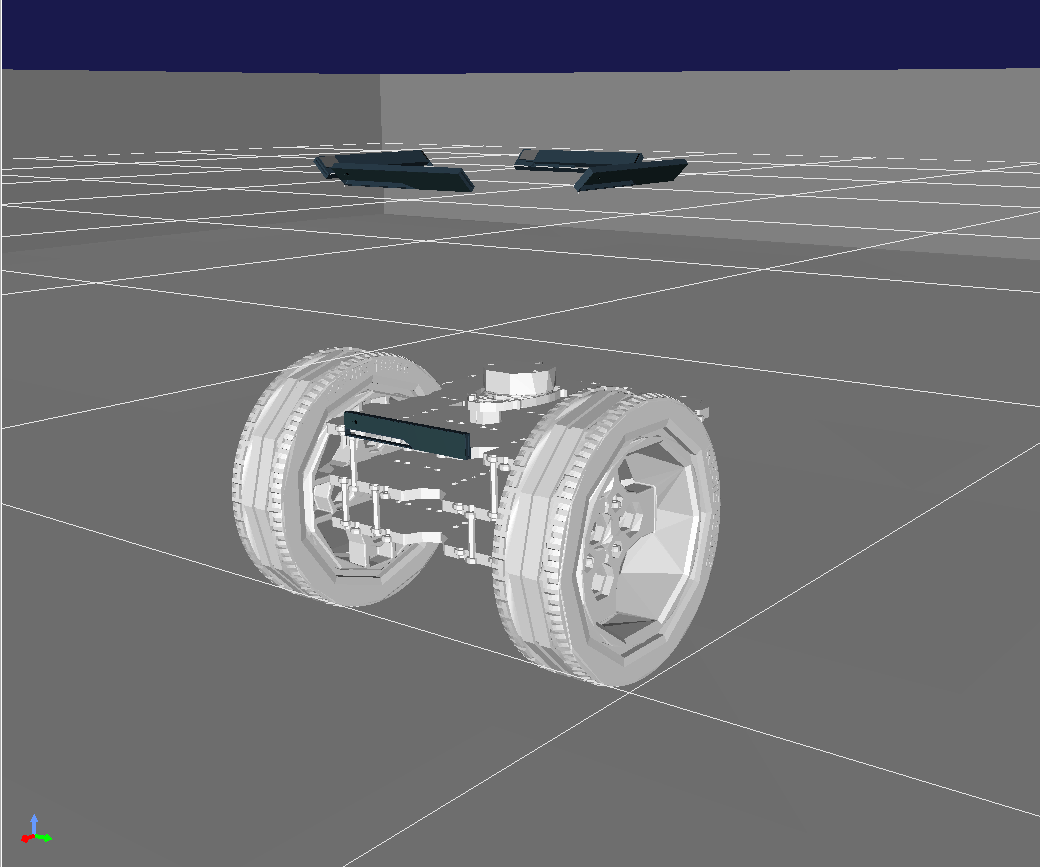
\includegraphics[width=0.4\linewidth]{images/robot_visual.png}
   \caption{ロボットの構成}
   \label{fig:fig}
  \end{center}
 \end{figure}


\begin{figure}[htbp]
  \begin{center}
   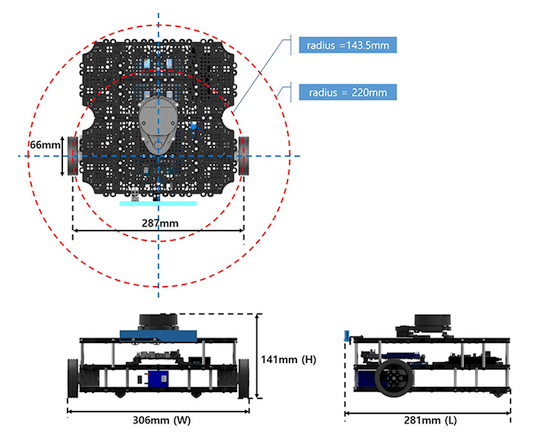
\includegraphics[width=0.7\linewidth]{images/turtlebot.png}
   \caption{TurtleBot3 Waffle}
   \label{fig:turtlebot}
  \end{center}
 \end{figure}

\subsection{走行計画手法}
走行計画として,4つの深度カメラから得られた画像から走行可能な方位を選択する方法を用いた.事前に生成した地形を用いて走行実験を行い,ある方位に走行可能だった場合はsafe(図\ref{fig:safe}) として 0,転倒や脱輪により探査続行不可になった場合はその直前の画像に danger(図\ref{fig:stack})として 1 をラベリングする.そのデータに対し出力が 0 から 1 になるよう機械学習し,走行中に推論した結果最も 0 に近い値を出力した方位に向かうようにした.例えば図\ref{fig:planning}のような場合には,ロボットは前方向に進む.
 \begin{figure}[htbp]
  \centering
  \begin{minipage}[b]{0.47\linewidth}
    \centering
    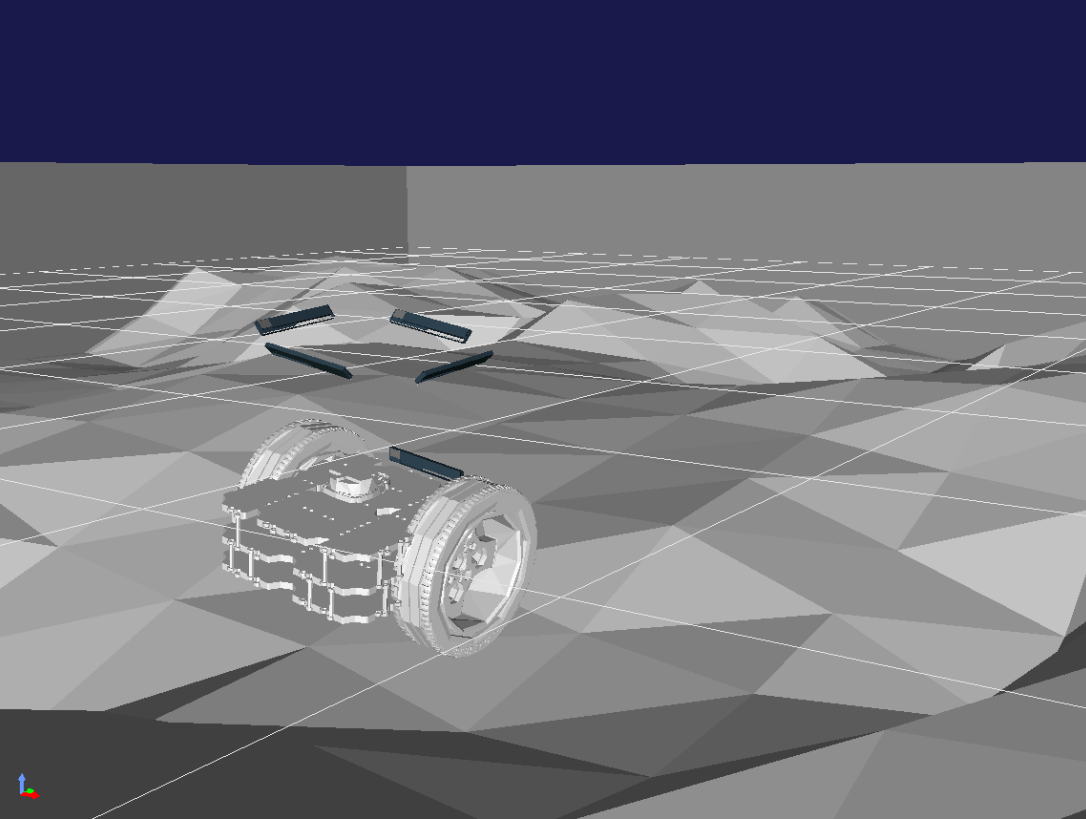
\includegraphics[keepaspectratio, scale=0.17]{images/safe.png}
    \subcaption{safeの時}\label{fig:safe}
  \end{minipage}
  \begin{minipage}[b]{0.47\linewidth}
    \centering
    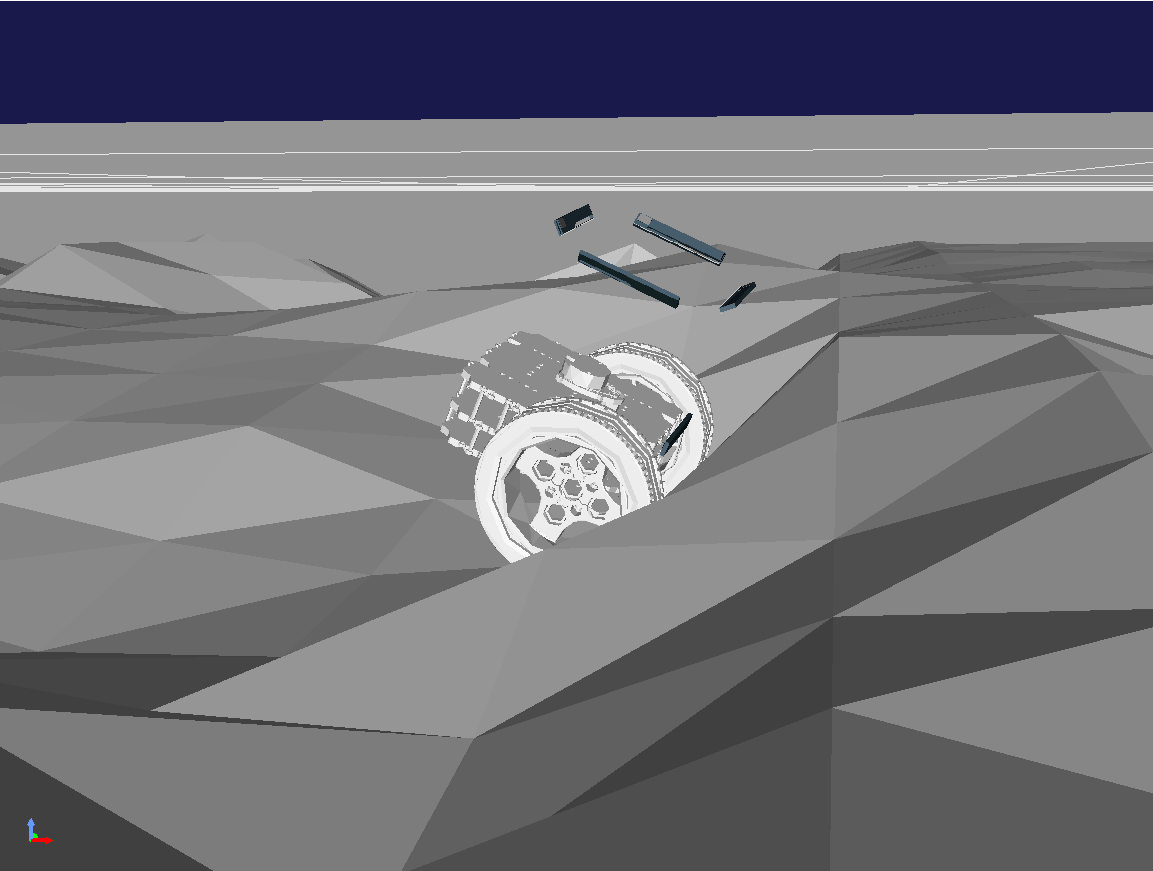
\includegraphics[keepaspectratio, scale=0.16]{images/stack.png}
    \subcaption{dangerの時}\label{fig:stack}
  \end{minipage}
  \caption{ラベリングのイメージ}
\end{figure}

\begin{figure}[htbp]
\begin{center}
  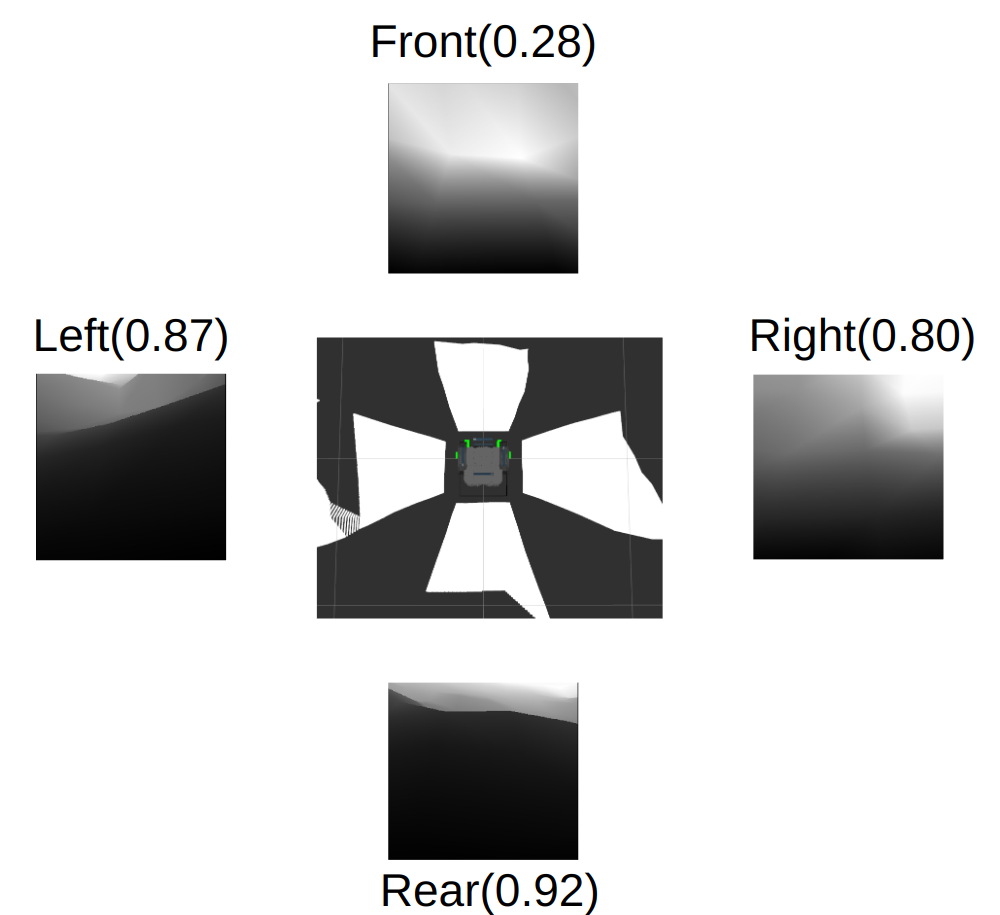
\includegraphics[width=0.6\linewidth]{images/planning.png}
  \caption{4方向からの深度画像と推論イメージ}
  \label{fig:planning}
\end{center}
\end{figure}

\subsection{実験方法}
予め生成した複数の不整地上を手動操作でロボットに走行させ,機械学習用データを収集する。画像数は計10000枚ほどであり,それぞれにsafeとdangerをラベリングした.学習モデルにはCNN(Convolutional Neural Network) を使用した.上記のデータを用いて学習を行い,再度生成した不整地上をロボットに走行させながらその軌跡を保存する.走行するマップ範囲内での軌跡の含有率をロボットの走破性と定義した.\cite{bunken2}シミュレーションにはロボット用統合 GUI ソフトウェアであるchoreonoid を用いた.このシミュレーション環境上に月面と$6 \mathrm{\,m}$\times$6\mathrm{\,m}$の壁を周囲に配置し,それをマップの範囲とした.[図\ref{fig:choreonoid}]

\begin{figure}[htbp]
  \begin{center}
   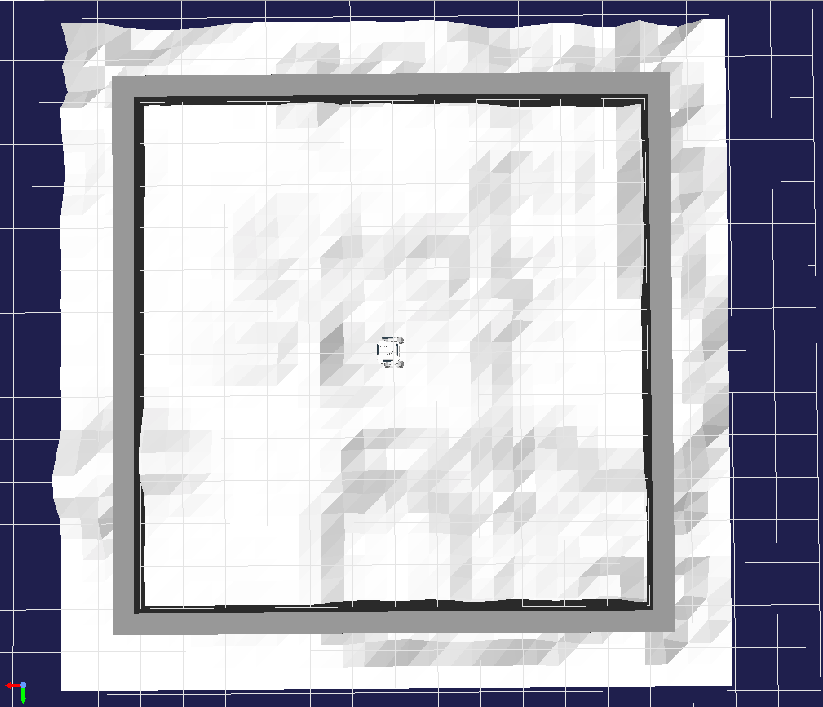
\includegraphics[width=0.5\linewidth]{images/choreonoid.png}
   \caption{実験用マップ}
   \label{fig:choreonoid}
  \end{center}
 \end{figure}

\subsection{生成地形の評価}
本研究では以下の2つの点からロボットを走行させることで地形データの評価をすることとした.
\begin{enumerate}
  \item 分散や標準偏差といった統計量が極端に離れている地形を生成した場合,特徴量の範囲が広い汎用的な地形データを収集できるが,学習用データとして用いて走行させた際に実際の地形に対する走破性向上に繋がるかは未知数となる.
  \item 仮に統計的に近い地形データを生成できたとしても,ロボットの座標や地表面のある隣接した領域どうしの関係性によって走破性は左右する.
\end{enumerate}
学習済みモデルを用いて,生成した不整地上と元の月面上をそれぞれ2分間走行させた際の軌跡に対し,マップの走破性を比較することで生成地形の有用性を評価した.使用した元の月面と生成した月面,走行した結果はそれぞれ下図のようになった.ここで,各グラフの中心がロボットの開始位置で,軌跡の止まった点がロボットの走行終了地点である.生成した地形の高さ方向の分散が起伏度合いに影響を与えるため,生成した月面2のような分散の小さいものを用いると極端に走破性が上がってしまった.逆に起伏が過度に激しいと,走破性が極端に下がり,かつロボットを配置したスタート地点に依存した走破性になってしまう.

\begin{figure}[htbp]
  \begin{center}
   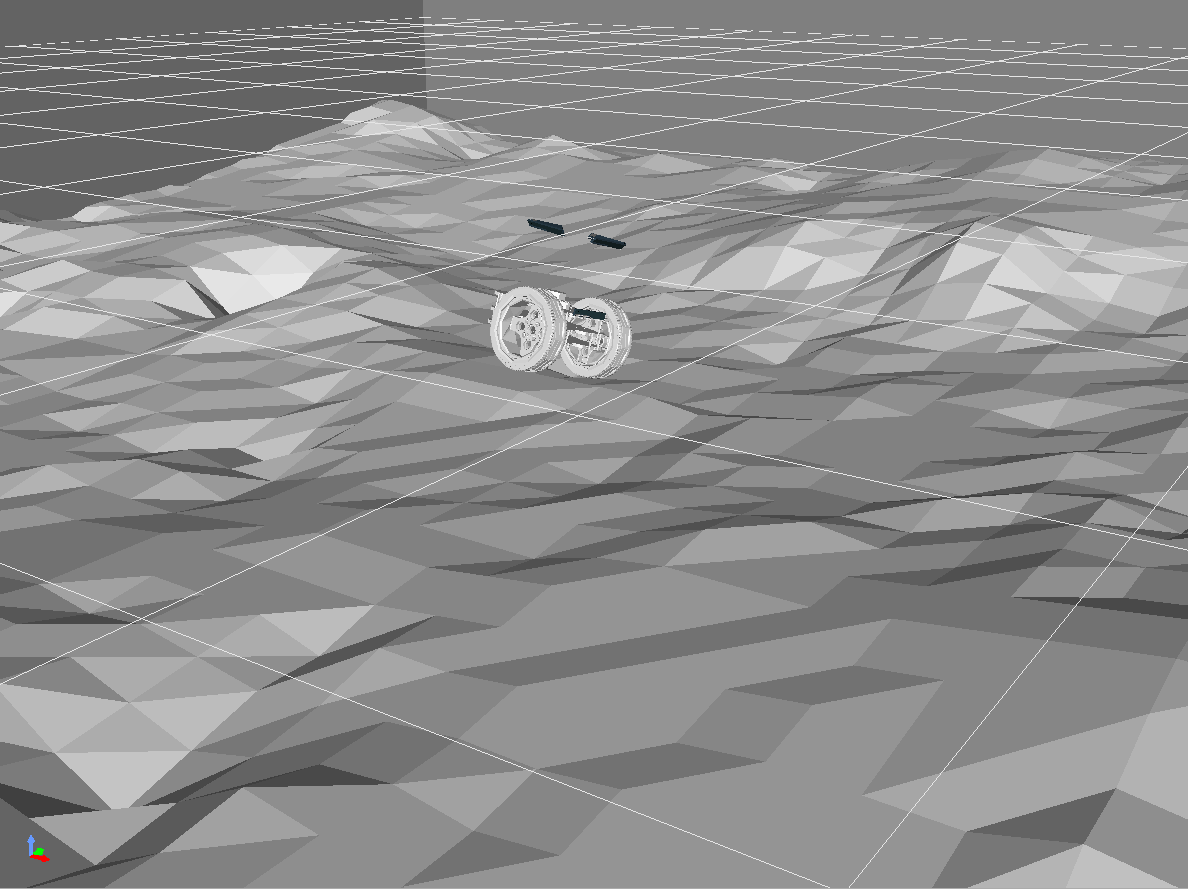
\includegraphics[width=0.6\linewidth]{images/test_field_origin1.png}
   \caption{元の月面1}
   \label{fig:test_field_origin1}
  \end{center}
 \end{figure}
 \begin{figure}[htbp]
  \begin{center}
   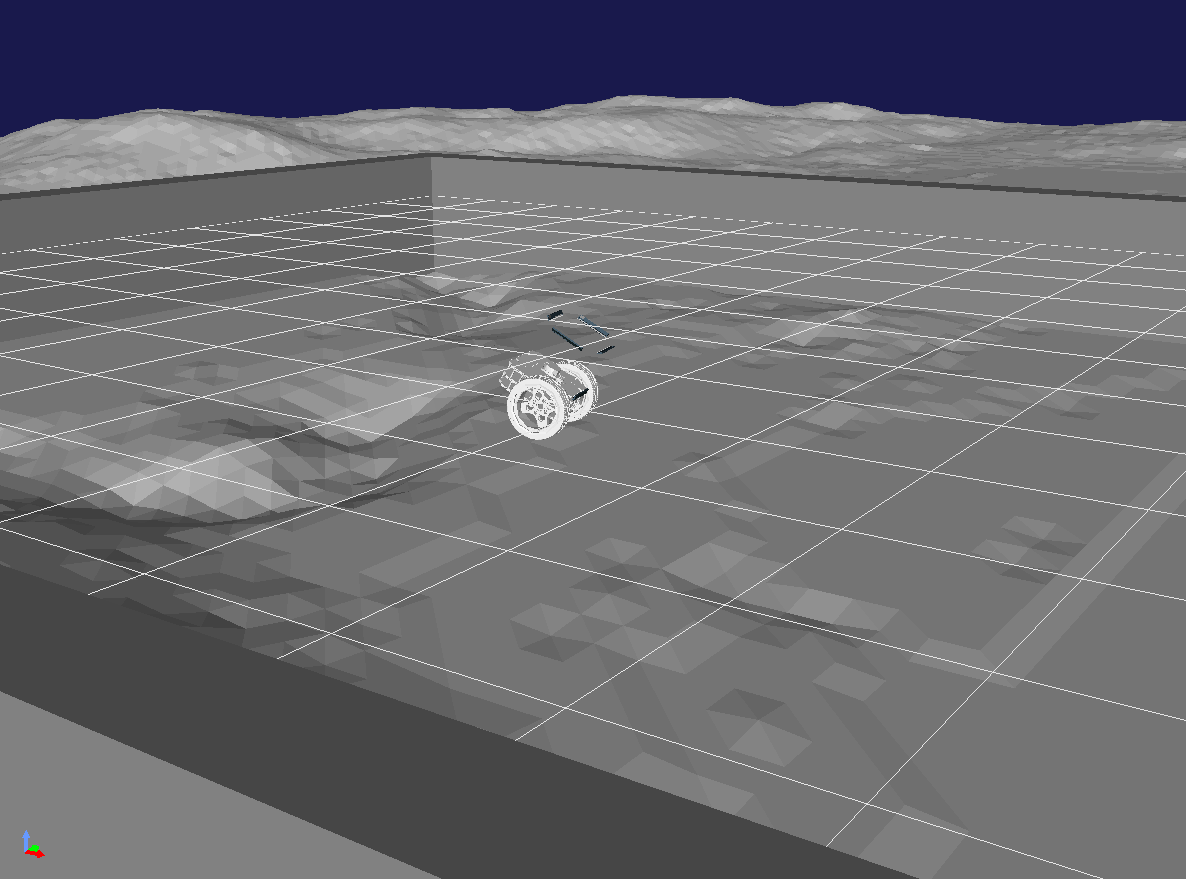
\includegraphics[width=0.6\linewidth]{images/test_field_origin2.png}
   \caption{元の月面2}
   \label{fig:test_field_origin2}
  \end{center}
 \end{figure}
 \begin{figure}[htbp]
  \begin{center}
   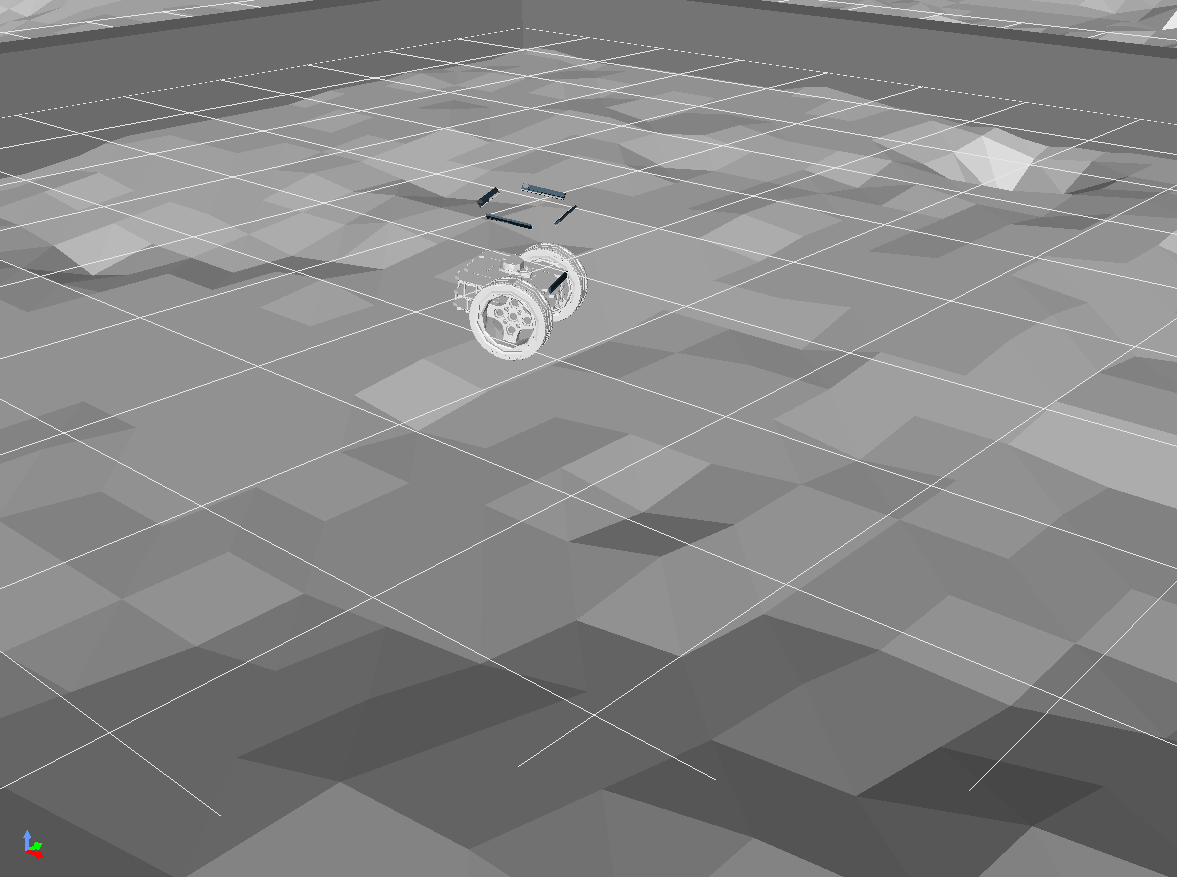
\includegraphics[width=0.6\linewidth]{images/origin_moon_field3.png}
   \caption{元の月面3}
   \label{fig:origin_moon_field3}
  \end{center}
 \end{figure}
 \begin{figure}[htbp]
  \begin{center}
   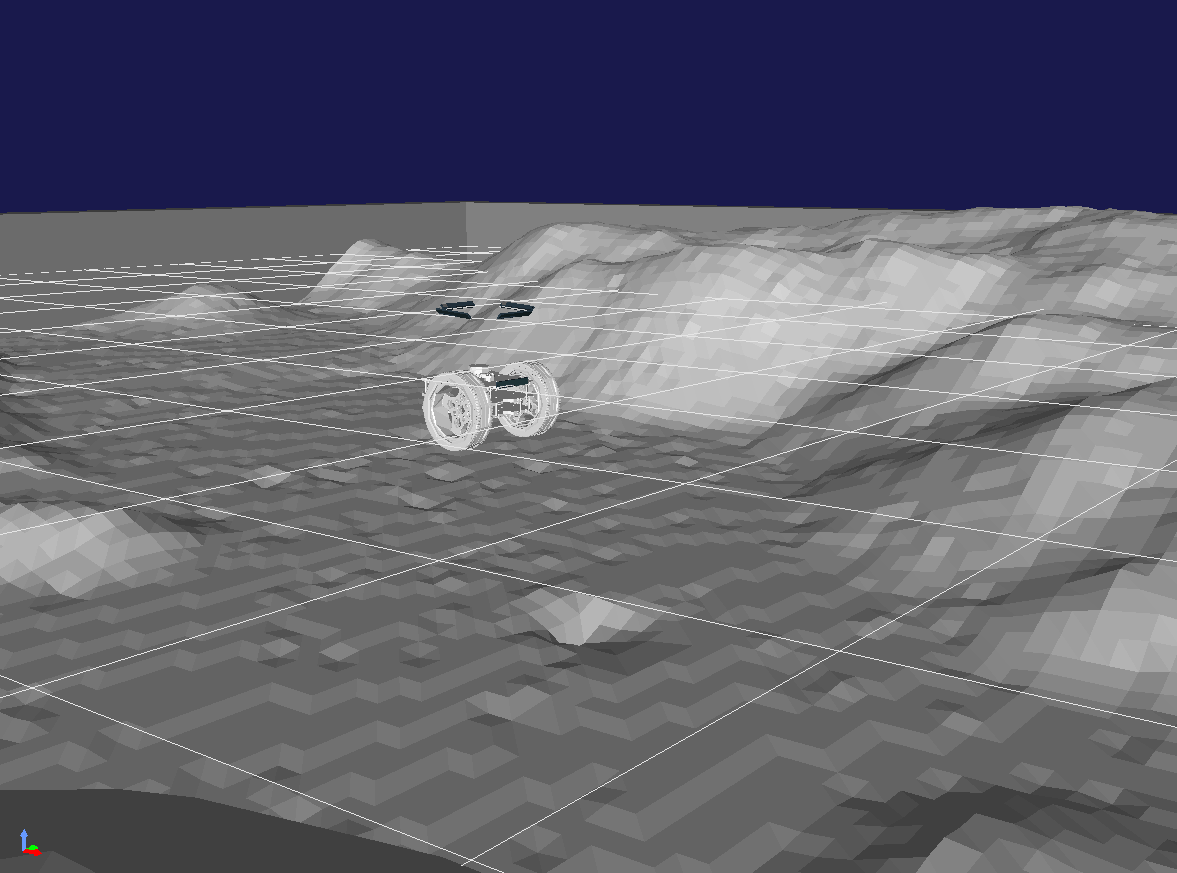
\includegraphics[width=0.6\linewidth]{images/original_moon_field4.png}
   \caption{元の月面4}
   \label{fig:original_moon_field4}
  \end{center}
 \end{figure}


% \begin{figure}[htbp]
%   \centering
  % \begin{minipage}[b]{0.48\linewidth}
  %   \centering
  %   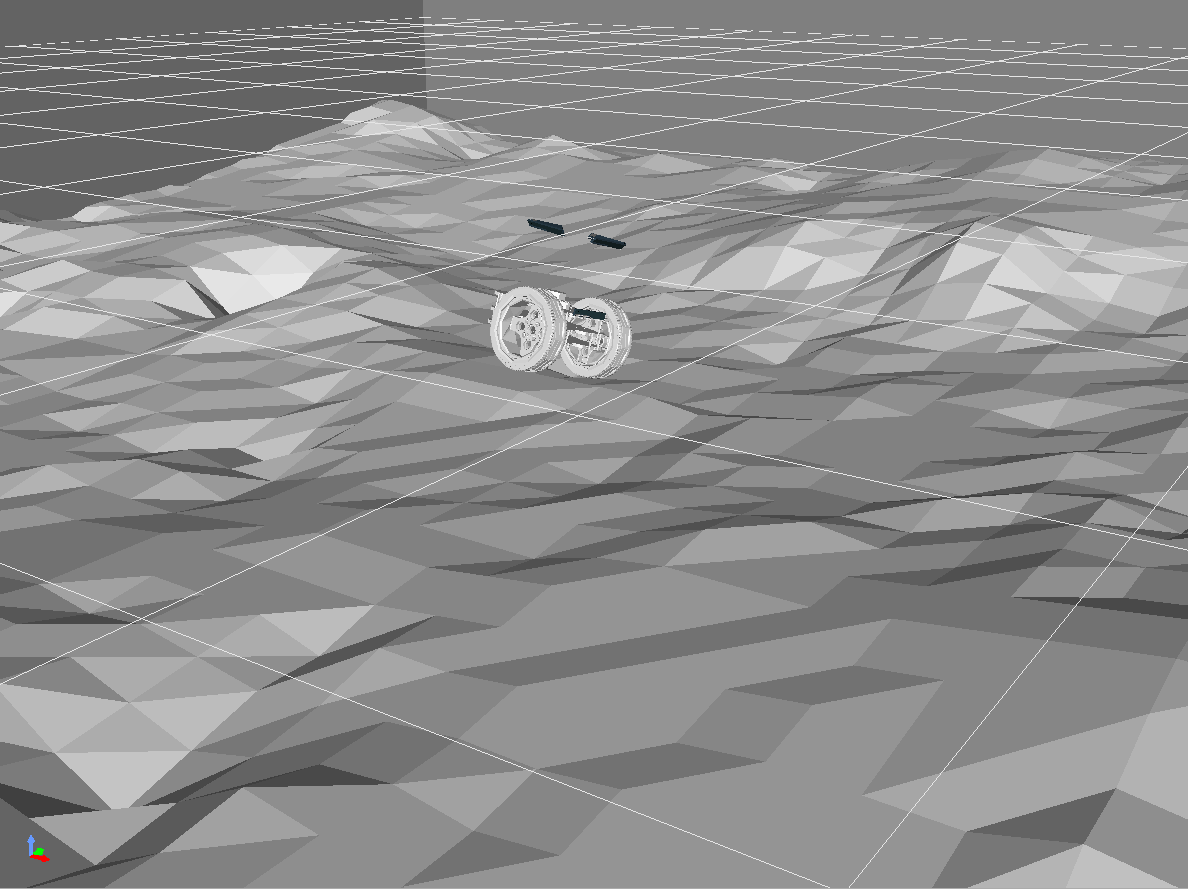
\includegraphics[keepaspectratio, scale=0.16]{images/test_field_origin1.png}
  %   \subcaption{元の月面1}\label{fig:test_field_origin1}
  % \end{minipage}
  % \begin{minipage}[b]{0.48\linewidth}
  %   \centering
  %   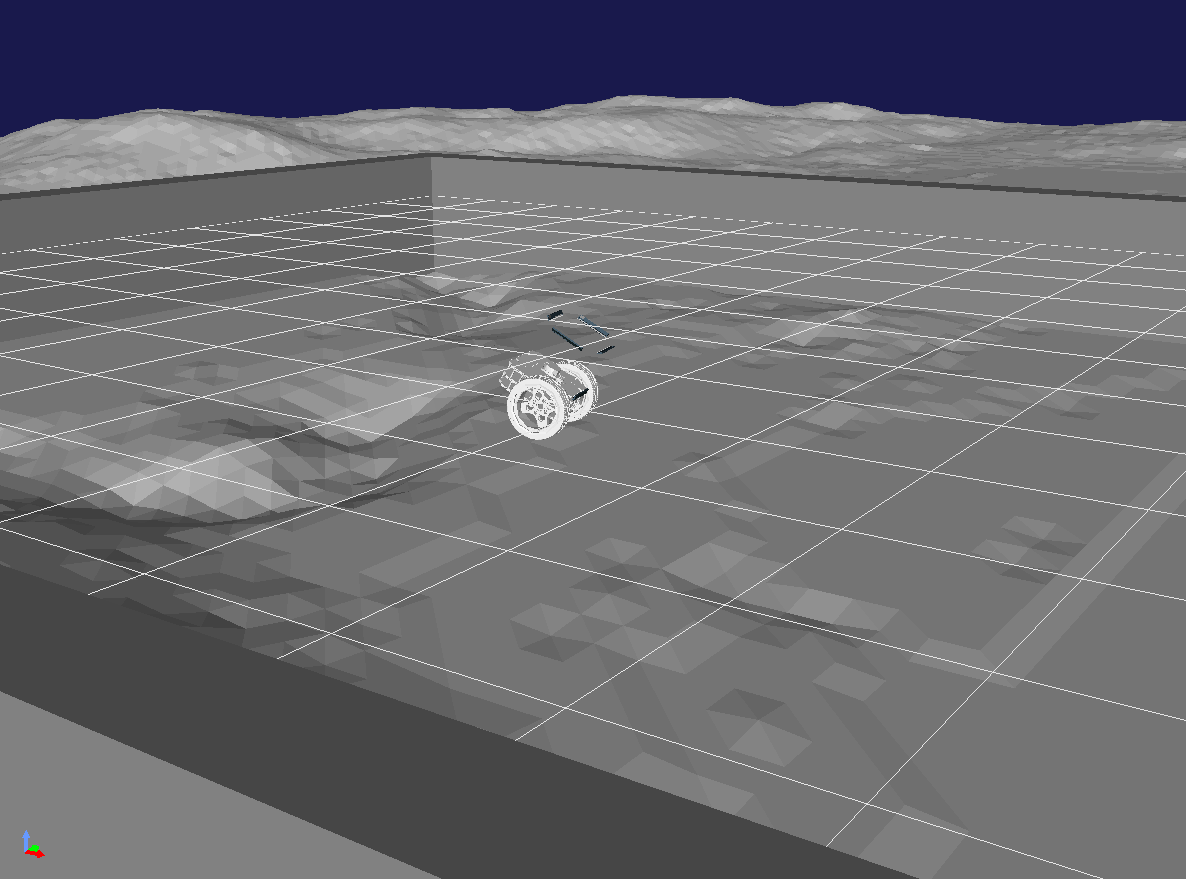
\includegraphics[keepaspectratio, scale=0.162]{images/test_field_origin2.png}
  %   \subcaption{元の月面2}\label{fig:test_field_origin2}
  % \end{minipage}
  % \begin{minipage}[b]{0.48\linewidth}
  %   \centering
  %   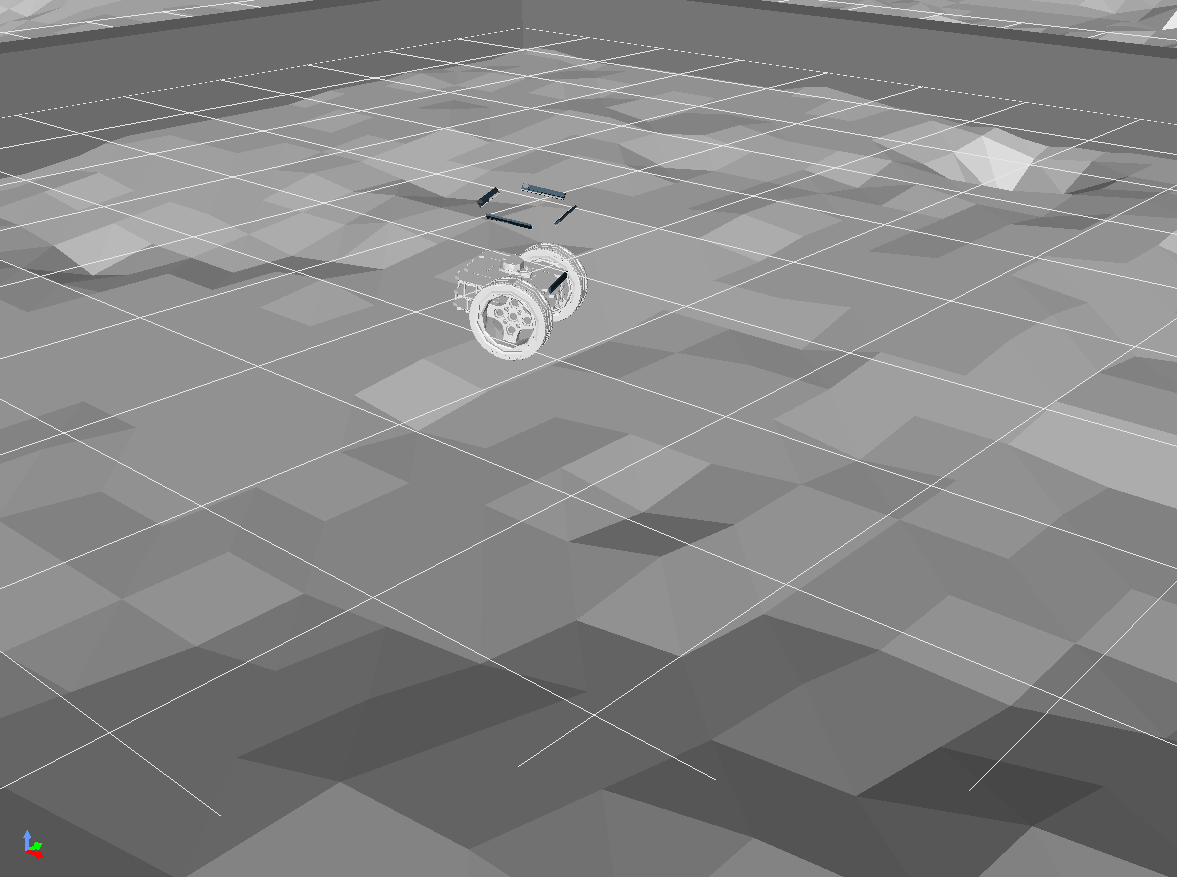
\includegraphics[keepaspectratio, scale=0.16]{images/origin_moon_field3.png}
  %   \subcaption{元の月面3}\label{fig:origin_moon_field3}
  % \end{minipage}
  % \begin{minipage}[b]{0.48\linewidth}
  %   \centering
  %   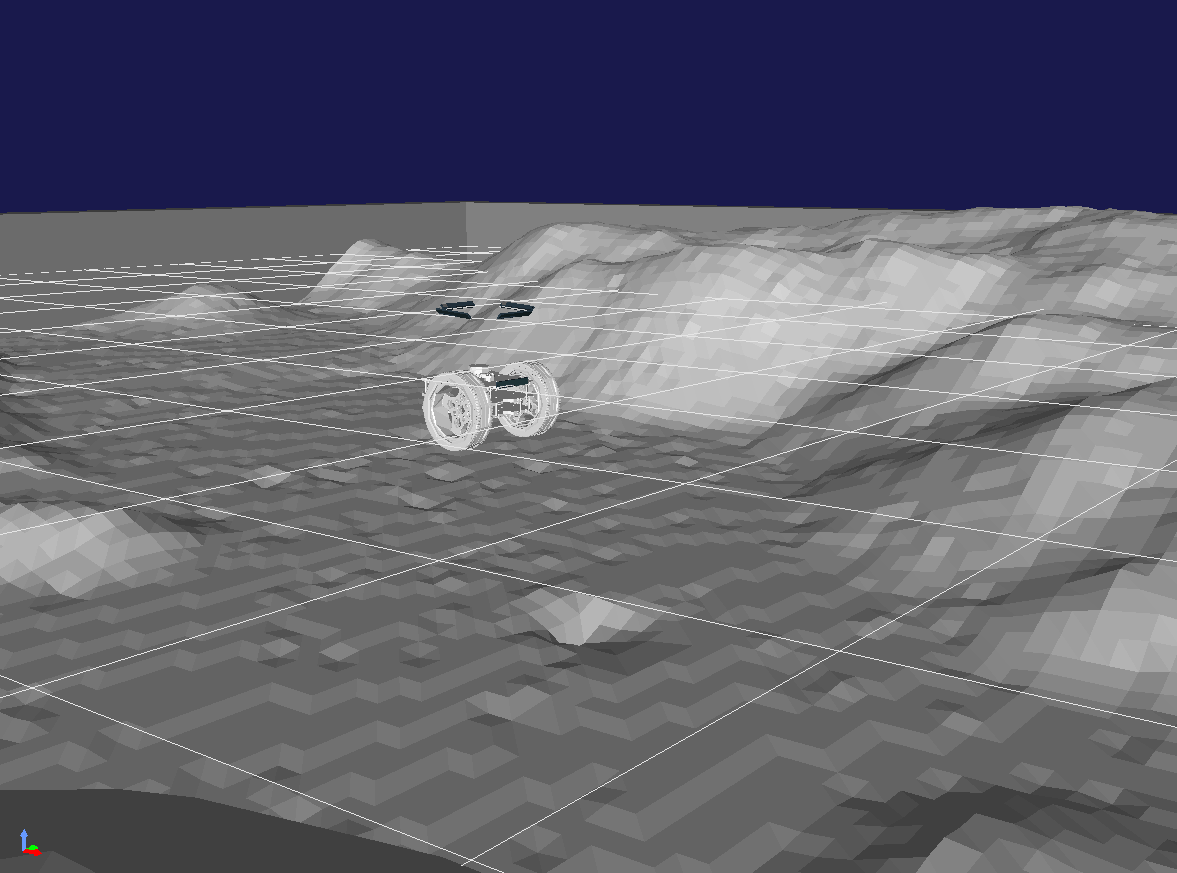
\includegraphics[keepaspectratio, scale=0.162]{images/original_moon_field4.png}
  %   \subcaption{元の月面4}\label{fig:origin_moon_field4}
  % \end{minipage}
% \end{figure}

\begin{figure}[htbp]
  \begin{center}
   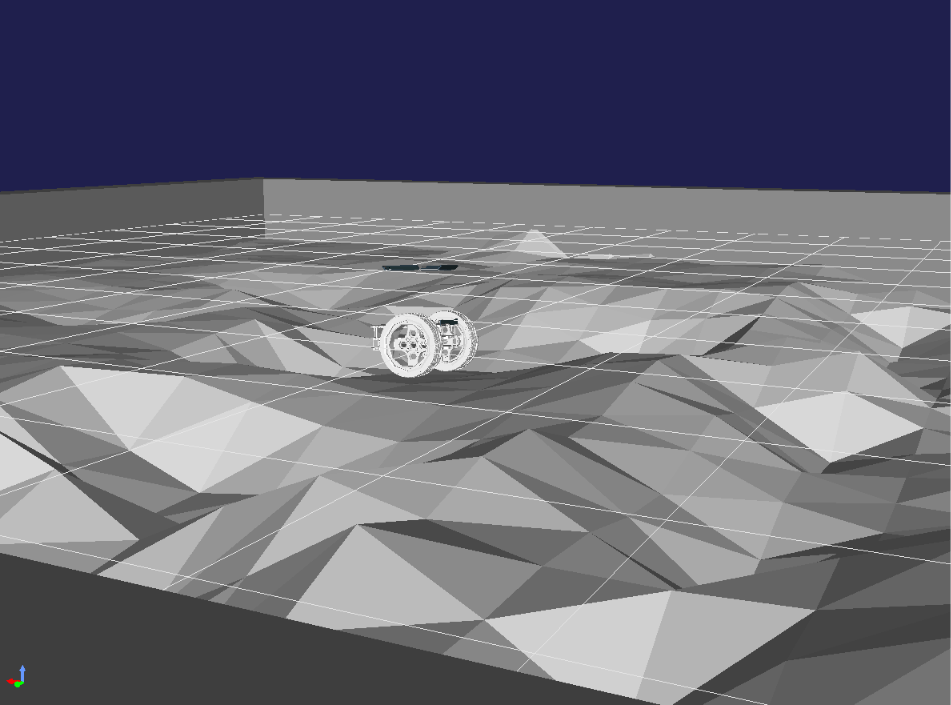
\includegraphics[width=0.6\linewidth]{images/test_field1.png}
   \caption{生成した月面1}
   \label{fig:test_field1}
  \end{center}
 \end{figure}
 \begin{figure}[htbp]
  \begin{center}
   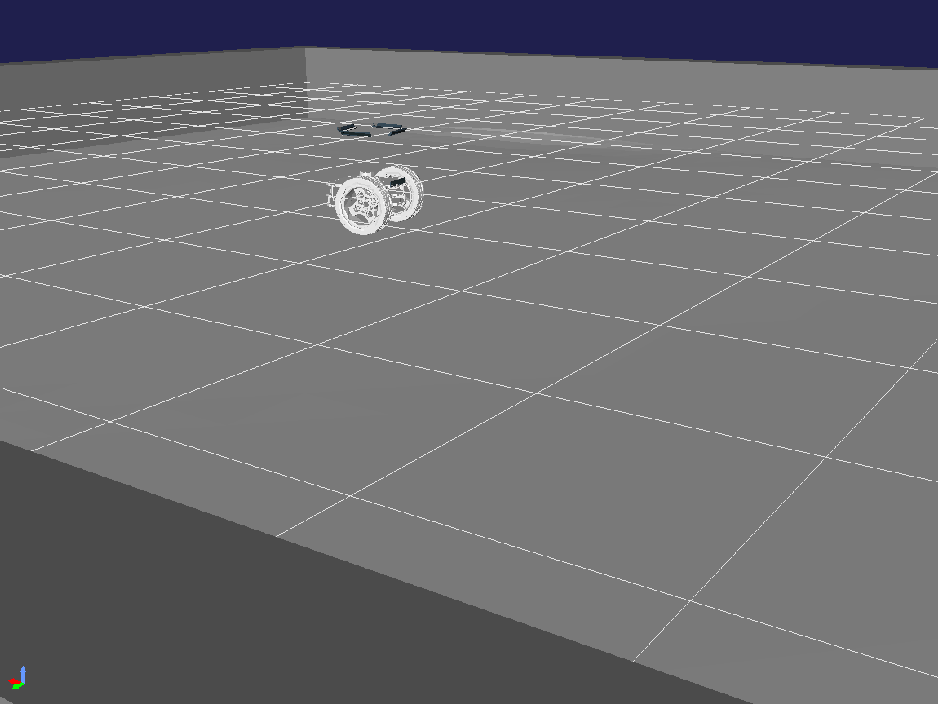
\includegraphics[width=0.6\linewidth]{images/test_field2.png}
   \caption{生成した月面2}
   \label{fig:test_field2}
  \end{center}
 \end{figure}
 \begin{figure}[htbp]
  \begin{center}
   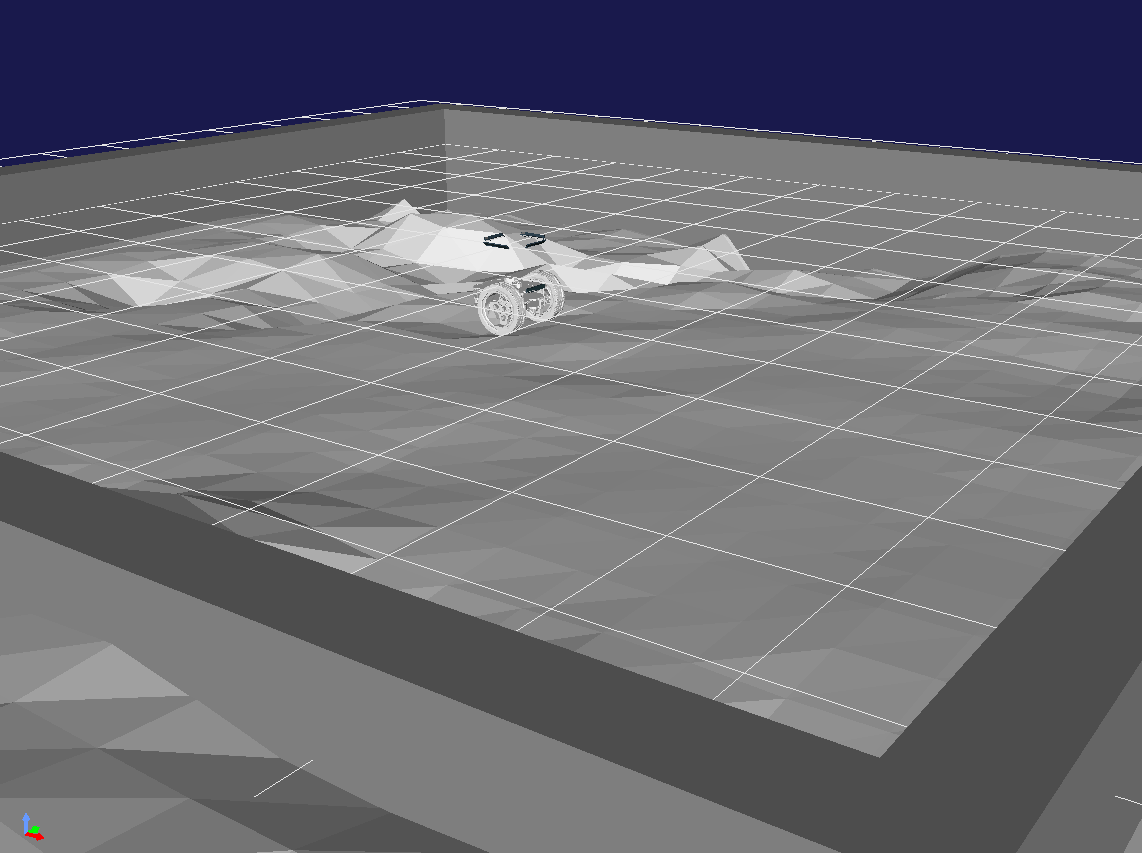
\includegraphics[width=0.6\linewidth]{images/generate_field3.png}
   \caption{生成した月面3}
   \label{fig:generate_field3}
  \end{center}
 \end{figure}
 \begin{figure}[htbp]
  \begin{center}
   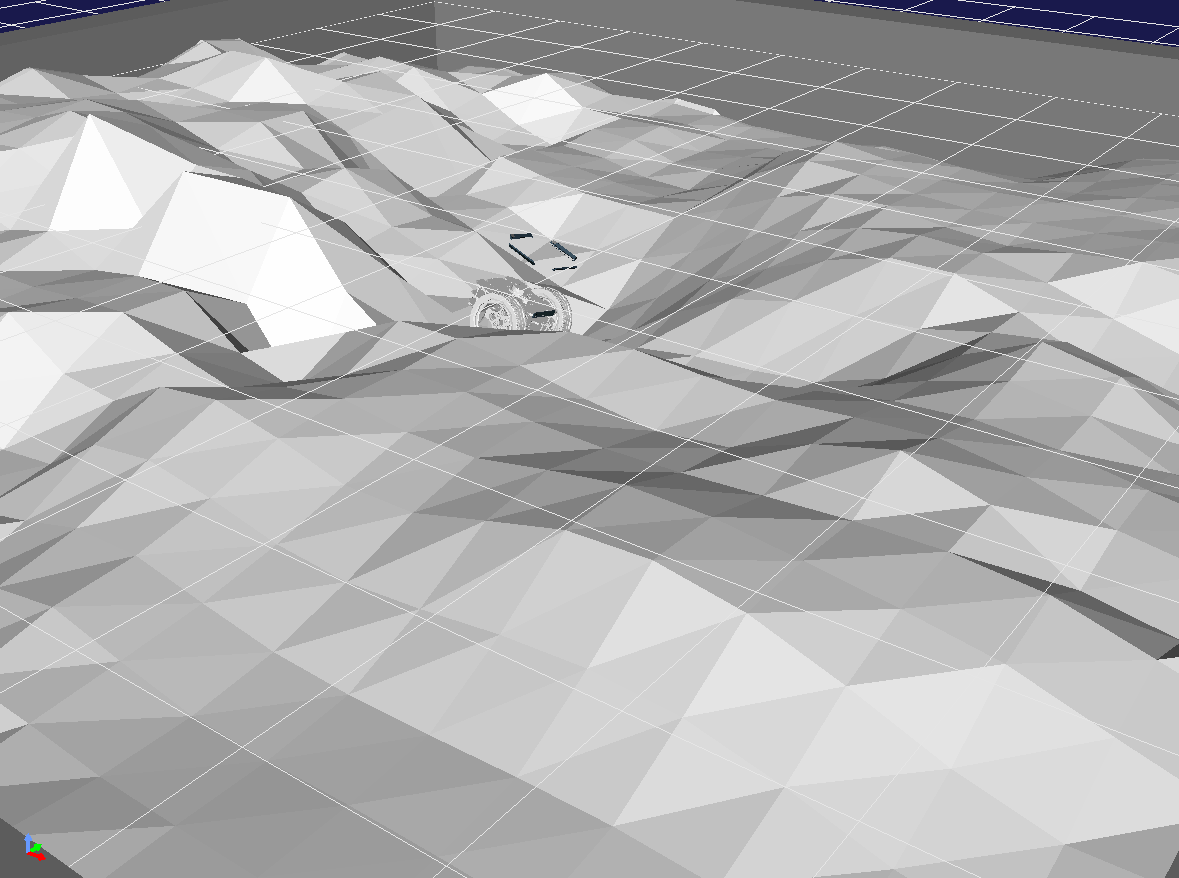
\includegraphics[width=0.6\linewidth]{images/generate_field4.png}
   \caption{生成した月面4}
   \label{fig:generate_field4}
  \end{center}
 \end{figure}

% \begin{figure}[htbp]
%   \begin{minipage}[b]{0.47\linewidth}
%     \centering
%     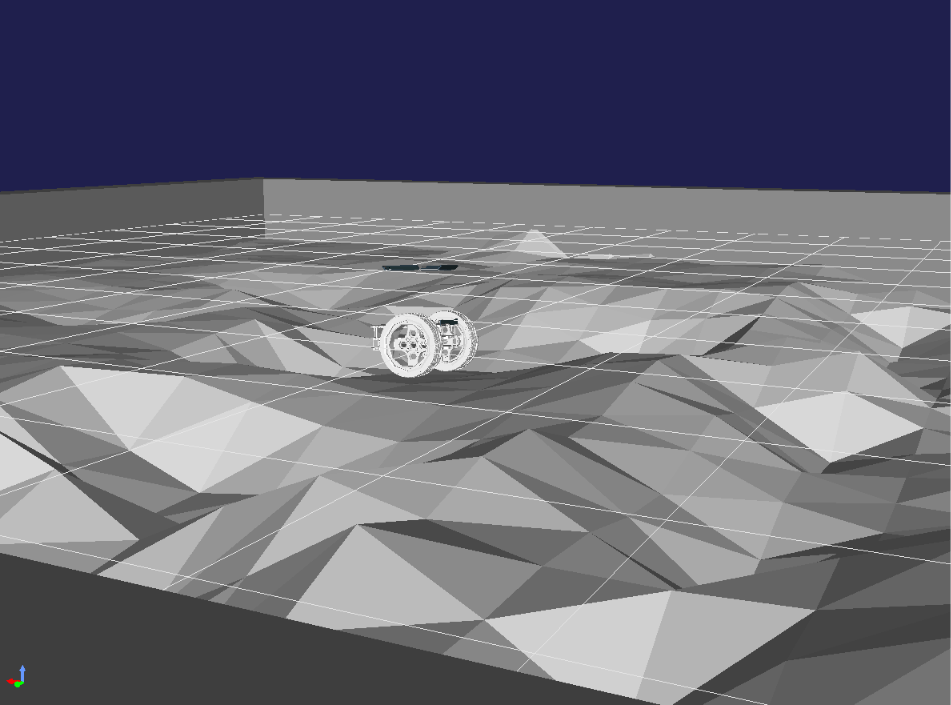
\includegraphics[keepaspectratio, scale=0.201]{images/test_field1.png}
%     \subcaption{生成した月面1}\label{fig:test_field1}
%   \end{minipage}
%   \begin{minipage}[b]{0.47\linewidth}
%     \centering
%     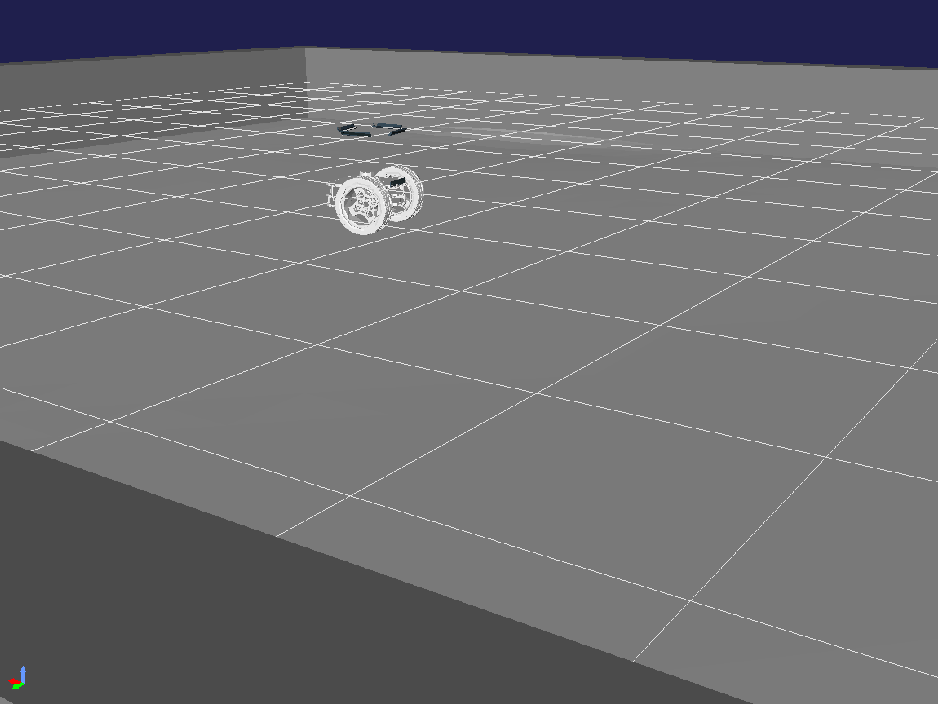
\includegraphics[keepaspectratio, scale=0.205]{images/test_field2.png}
%     \subcaption{生成した月面2}\label{fig:test_field2}
%   \end{minipage}
%   \begin{minipage}[b]{0.6\linewidth}
%     \centering
%     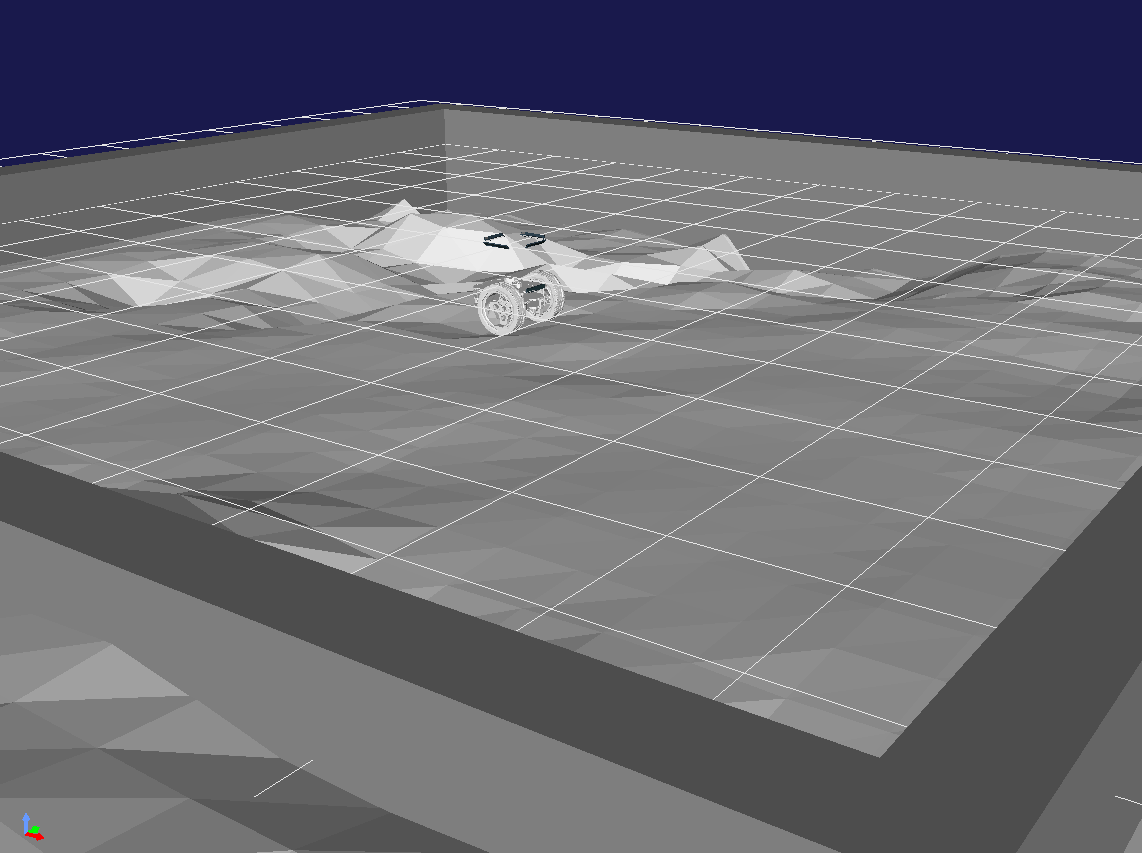
\includegraphics[keepaspectratio, scale=0.173]{images/generate_field3.png}
%     \subcaption{生成した月面3}\label{fig:generate_field3}
%   \end{minipage}
%   \begin{minipage}[b]{0.6\linewidth}
%     \centering
%     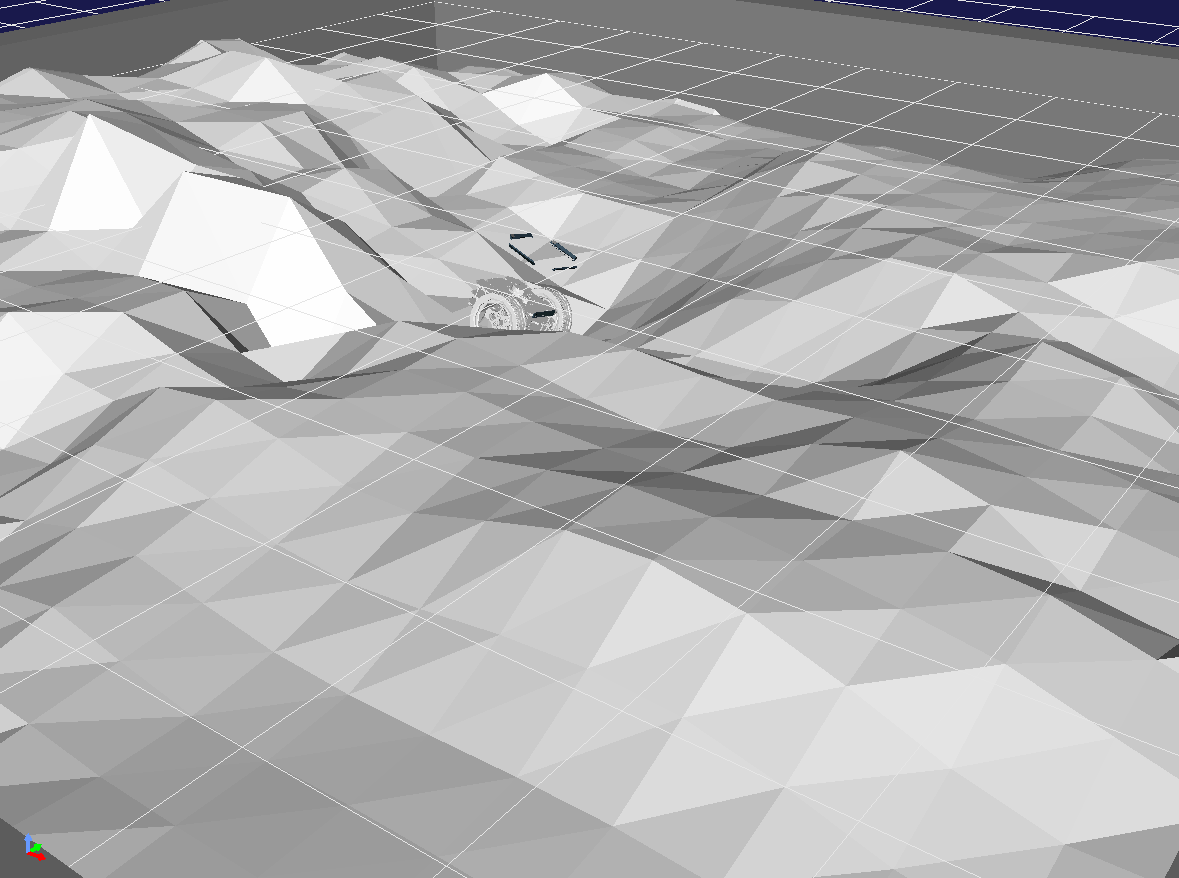
\includegraphics[keepaspectratio, scale=0.17]{images/generate_field4.png}
%     \subcaption{生成した月面4}\label{fig:generate_field4}
%   \end{minipage}
%   \caption{使用した月面の種類}\label{fig:fields}
% \end{figure}

\begin{figure}[htbp]
  \begin{center}
   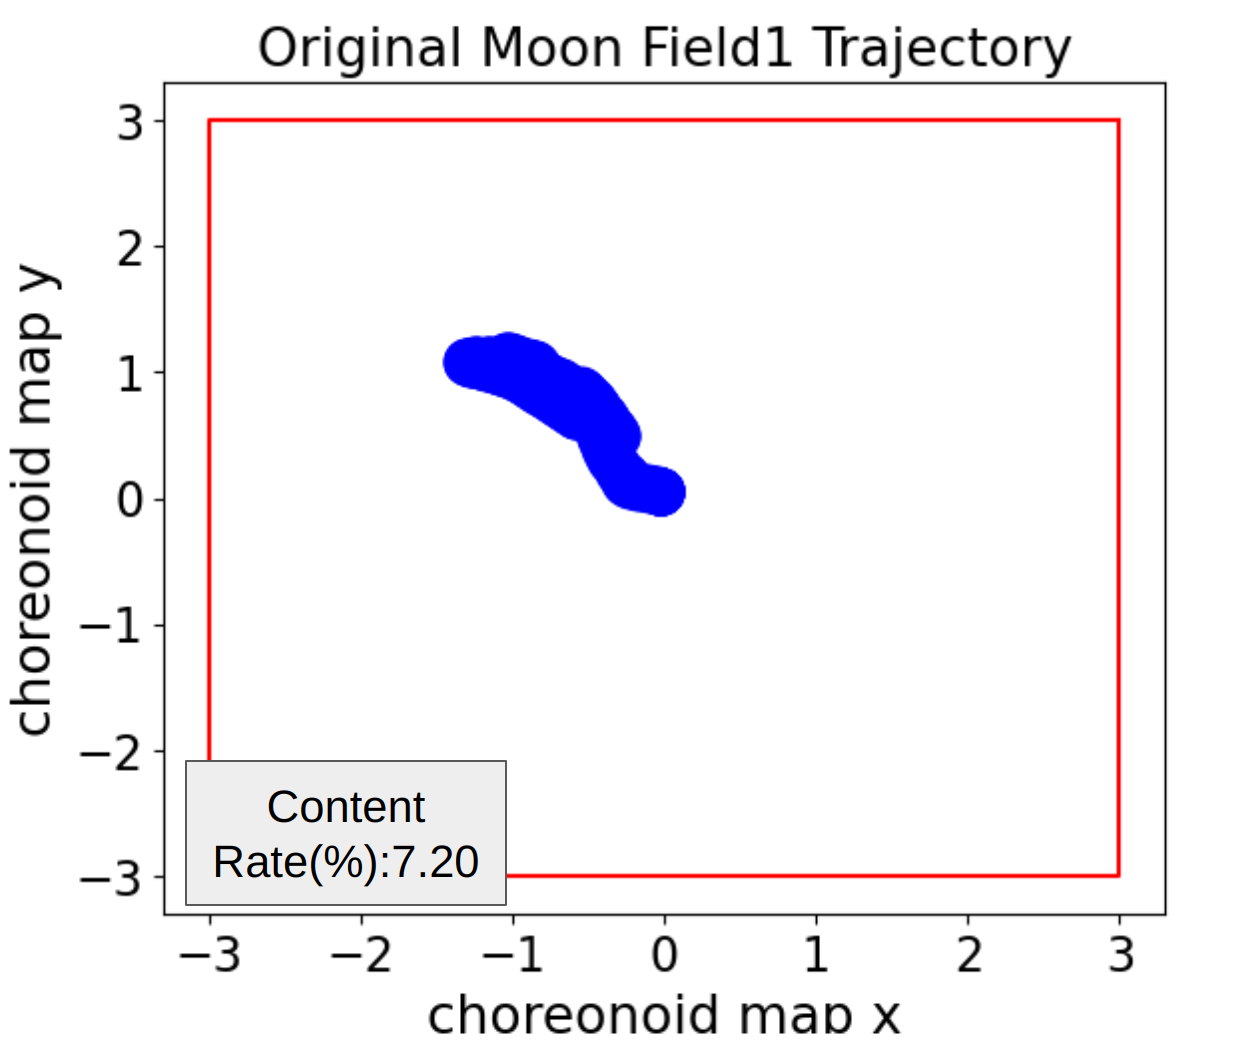
\includegraphics[width=0.6\linewidth]{images/origin_moon_field1.png}
   \caption{元の月面1}
   \label{fig:origin_moon_field1}
  \end{center}
 \end{figure}
 \begin{figure}[htbp]
  \begin{center}
   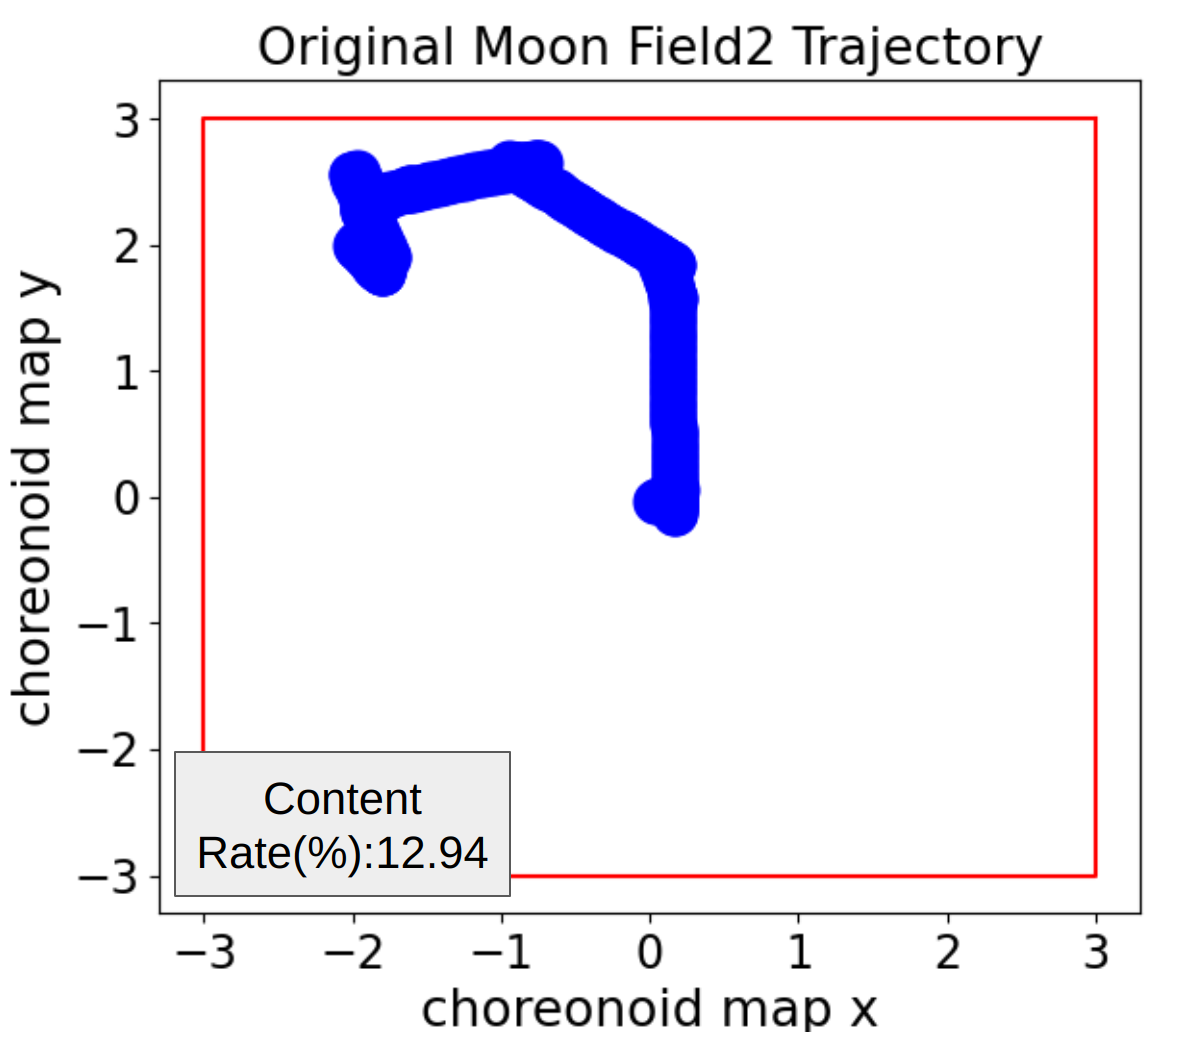
\includegraphics[width=0.6\linewidth]{images/origin_moon_field2.png}
   \caption{元の月面2}
   \label{fig:origin_moon_field2}
  \end{center}
 \end{figure}
 \begin{figure}[htbp]
  \begin{center}
   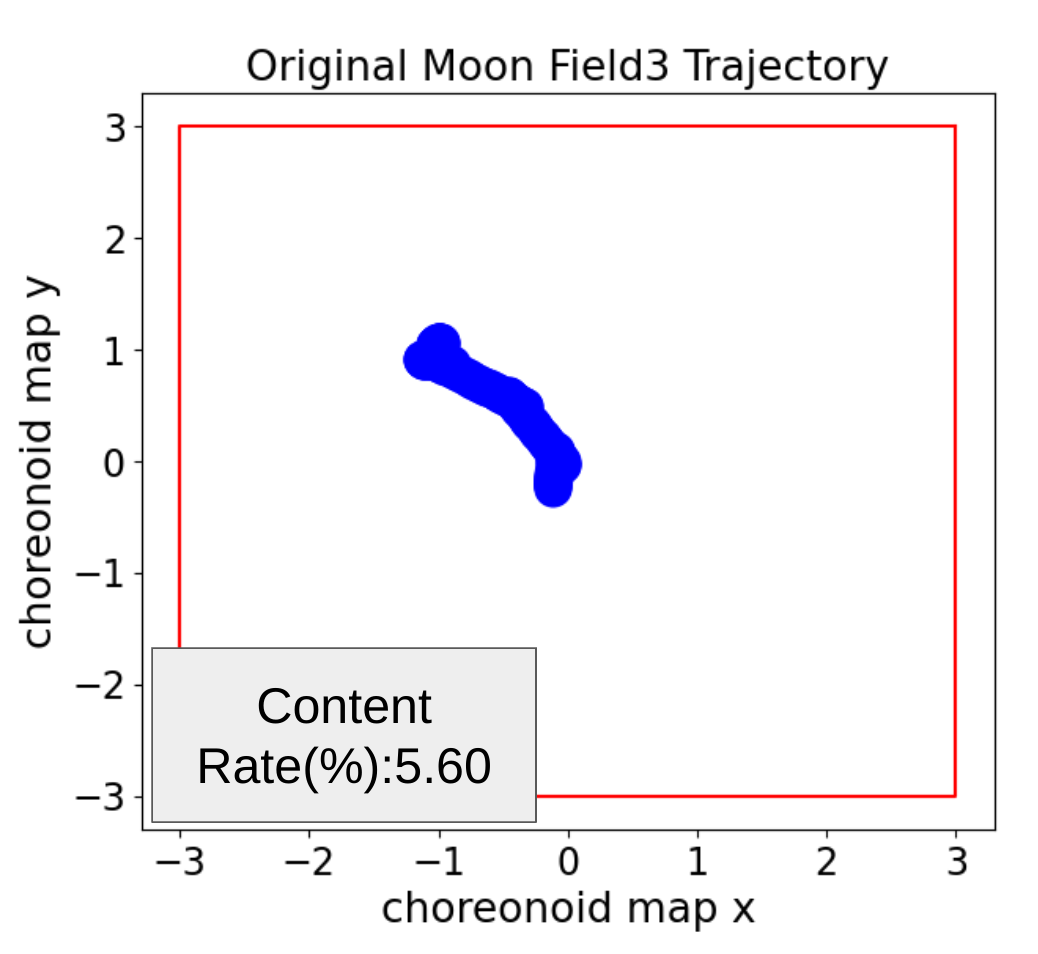
\includegraphics[width=0.6\linewidth]{images/origin_moon_trajectory3.png}
   \caption{元の月面3}
   \label{fig:origin_moon_trajectory3}
  \end{center}
 \end{figure}
 \begin{figure}[htbp]
  \begin{center}
   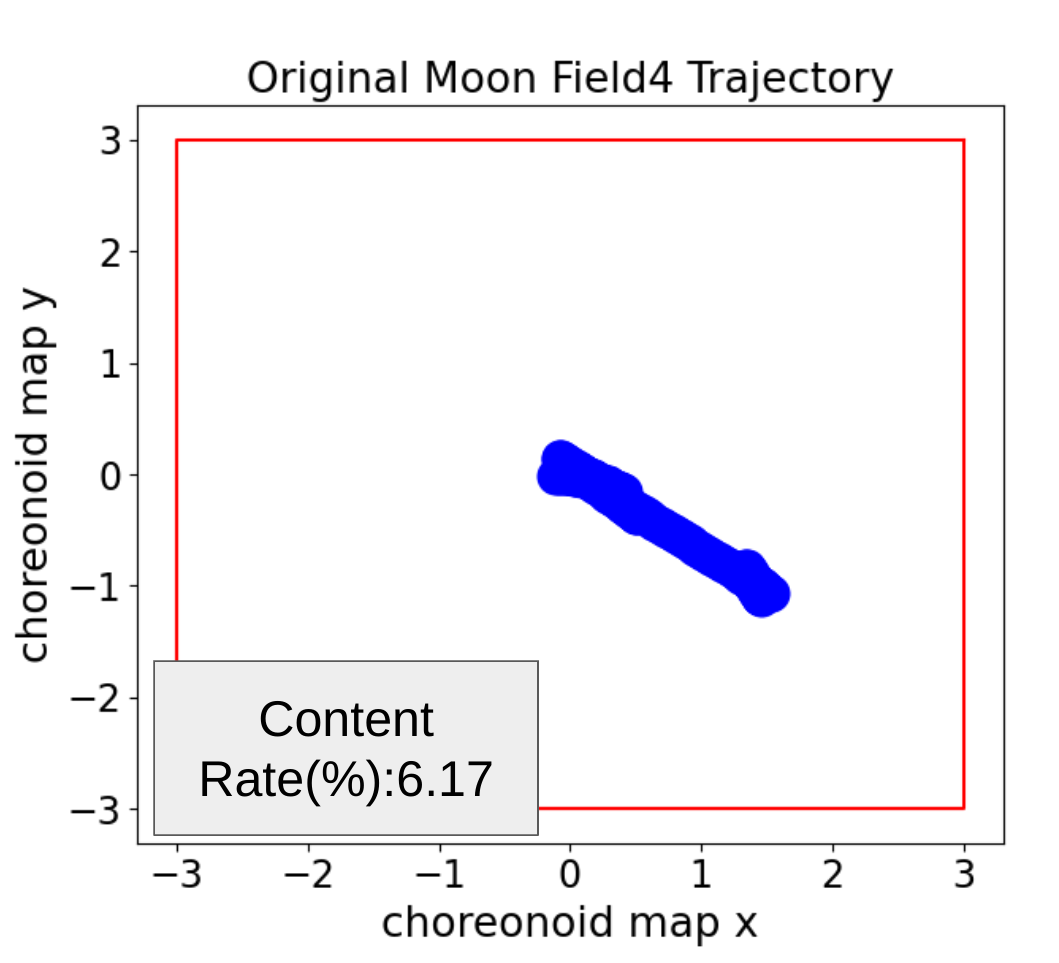
\includegraphics[width=0.6\linewidth]{images/origin_moon_trajectory4.png}
   \caption{元の月面4}
   \label{fig:origin_moon_trajectory4}
  \end{center}
 \end{figure}

% \begin{figure}[htbp]
%   \centering
%   \begin{minipage}[b]{0.48\linewidth}
%     \centering
%     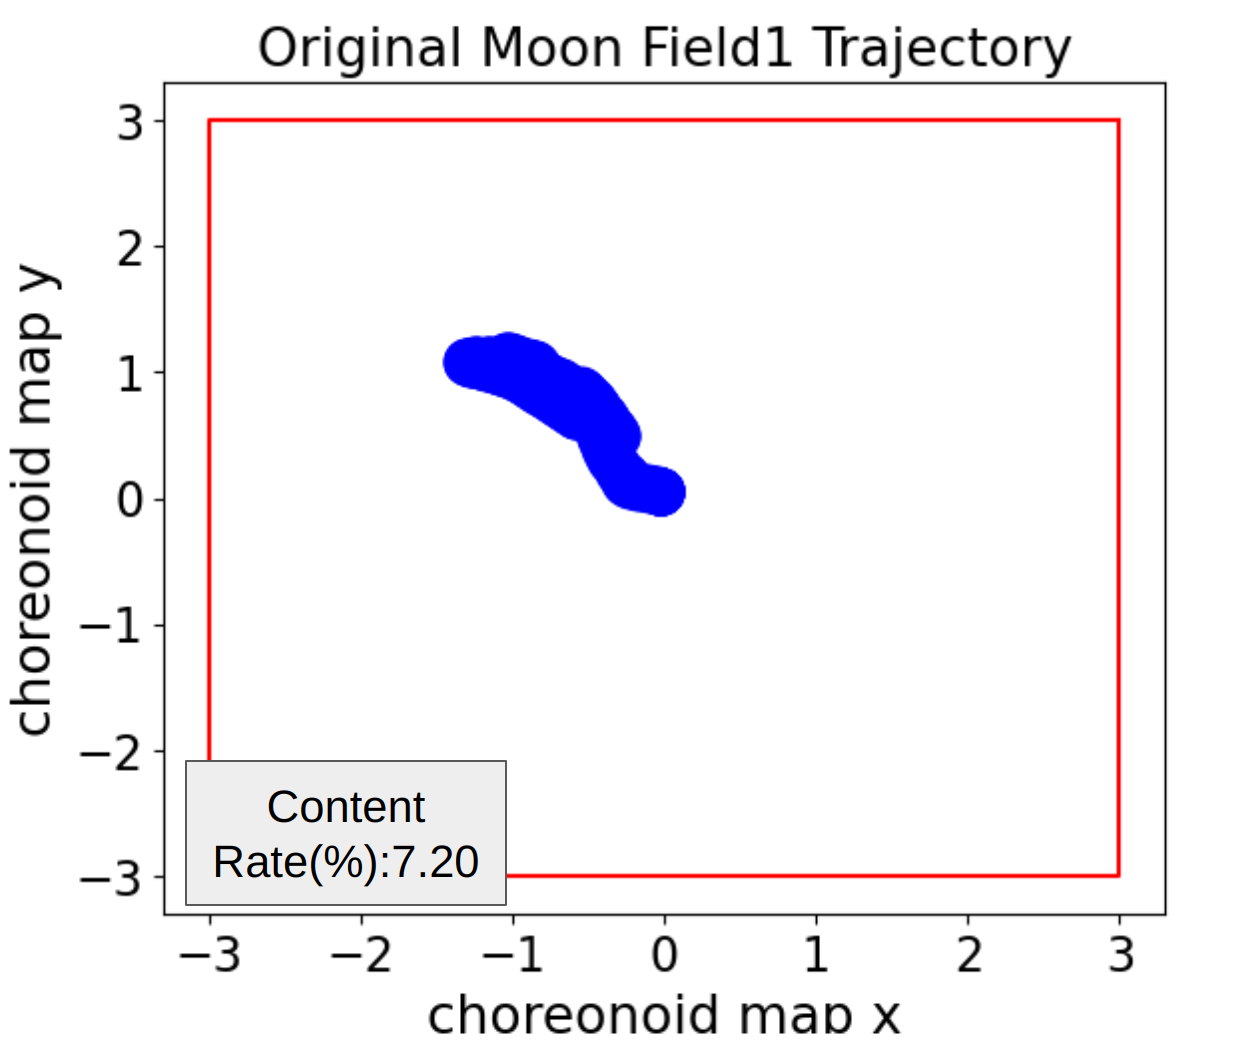
\includegraphics[keepaspectratio, scale=0.165]{images/origin_moon_field1.png}
%     \subcaption{元の月面1}\label{fig:origin_moon_field1}
%   \end{minipage}
%   \begin{minipage}[b]{0.48\linewidth}
%     \centering
%     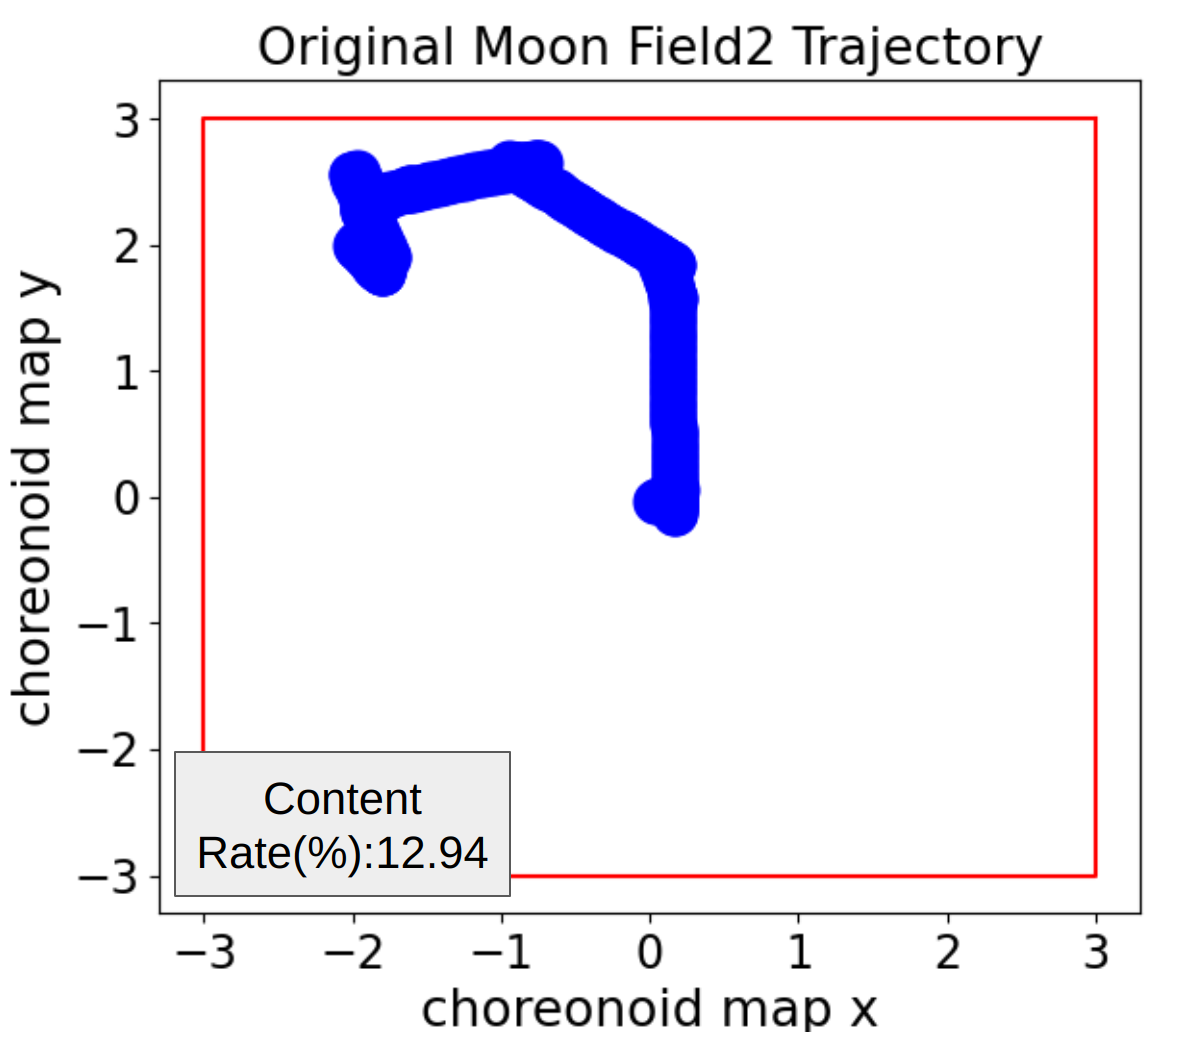
\includegraphics[keepaspectratio, scale=0.167]{images/origin_moon_field2.png}
%     \subcaption{元の月面2}\label{fig:origin_moon_field2}
%   \end{minipage}
%   \begin{minipage}[b]{0.49\linewidth}
%     \centering
%     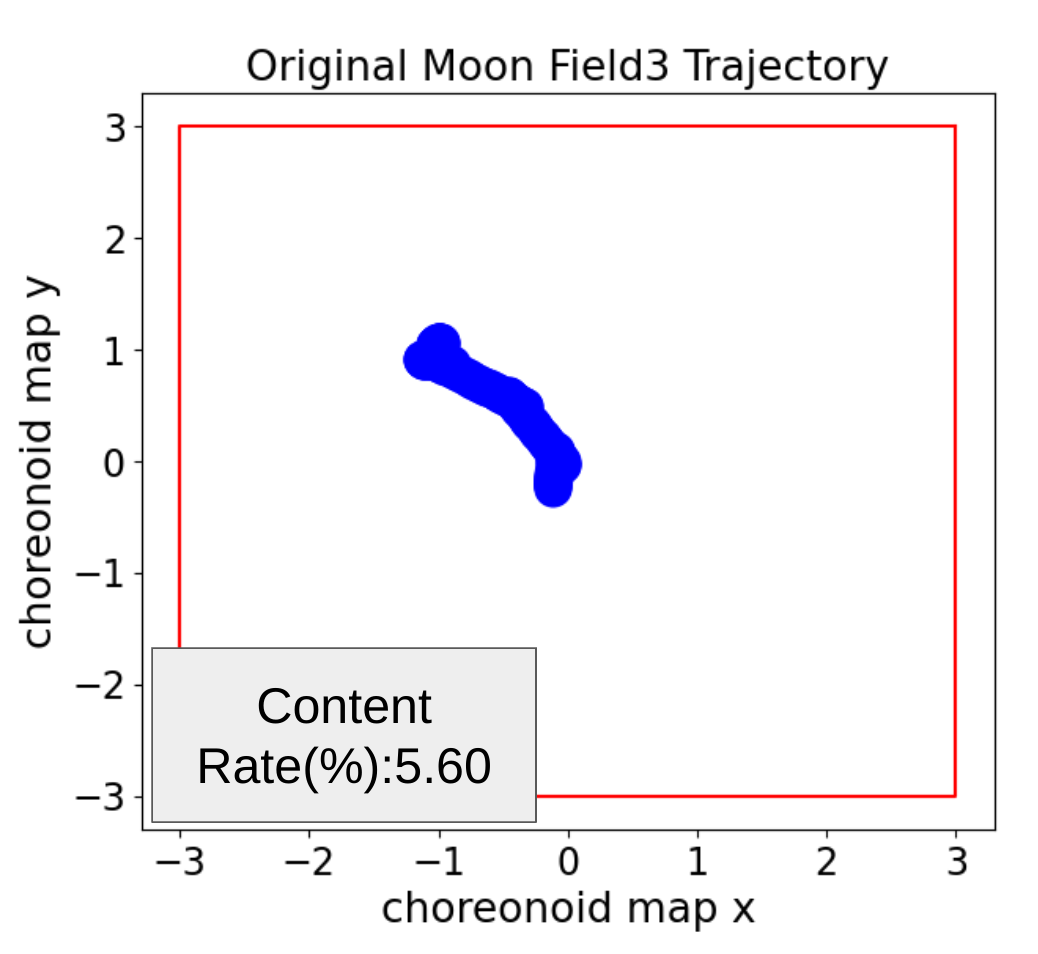
\includegraphics[keepaspectratio, scale=0.165]{images/origin_moon_trajectory3.png}
%     \subcaption{元の月面3}\label{fig:origin_moon_trajectory3}
%   \end{minipage}
%   \begin{minipage}[b]{0.49\linewidth}
%     \centering
%     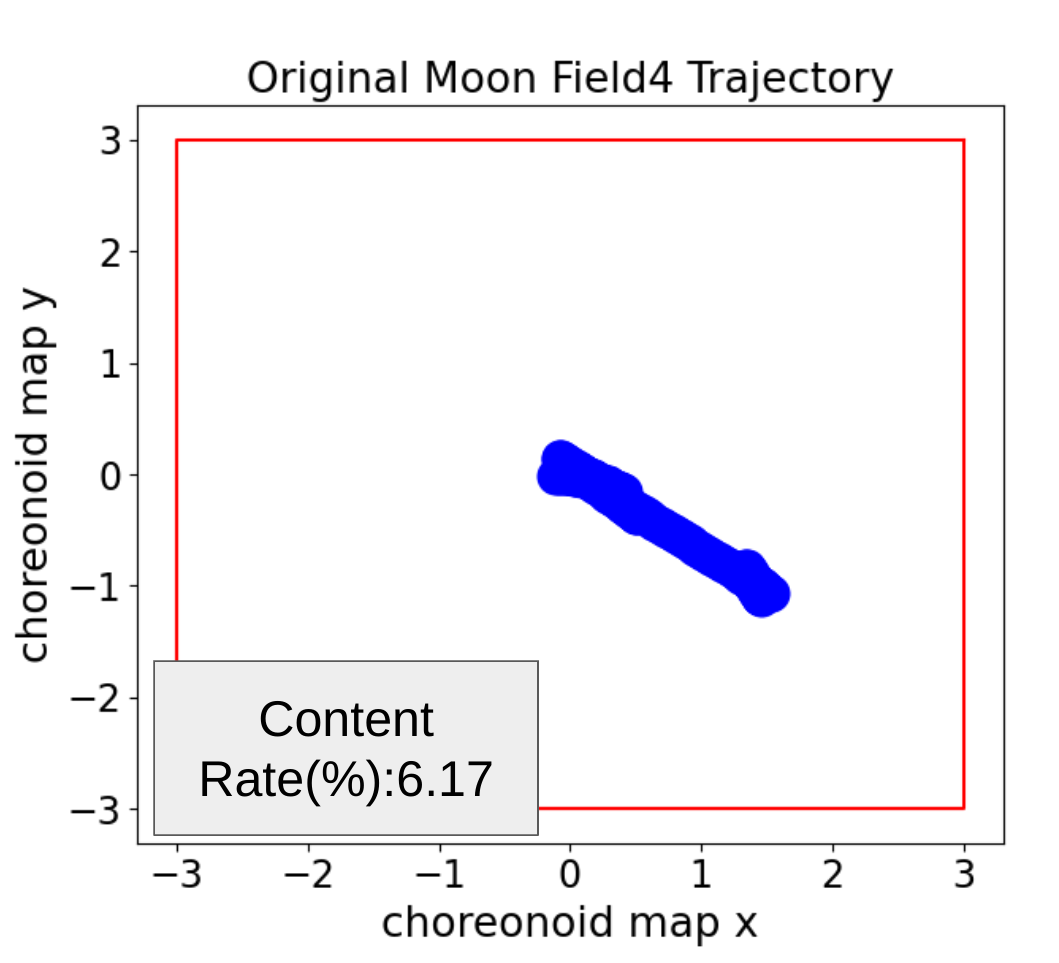
\includegraphics[keepaspectratio, scale=0.165]{images/origin_moon_trajectory4.png}
%     \subcaption{元の月面4}\label{fig:origin_moon_trajectory4}
%   \end{minipage}
% \end{figure}

\begin{figure}[htbp]
  \begin{center}
   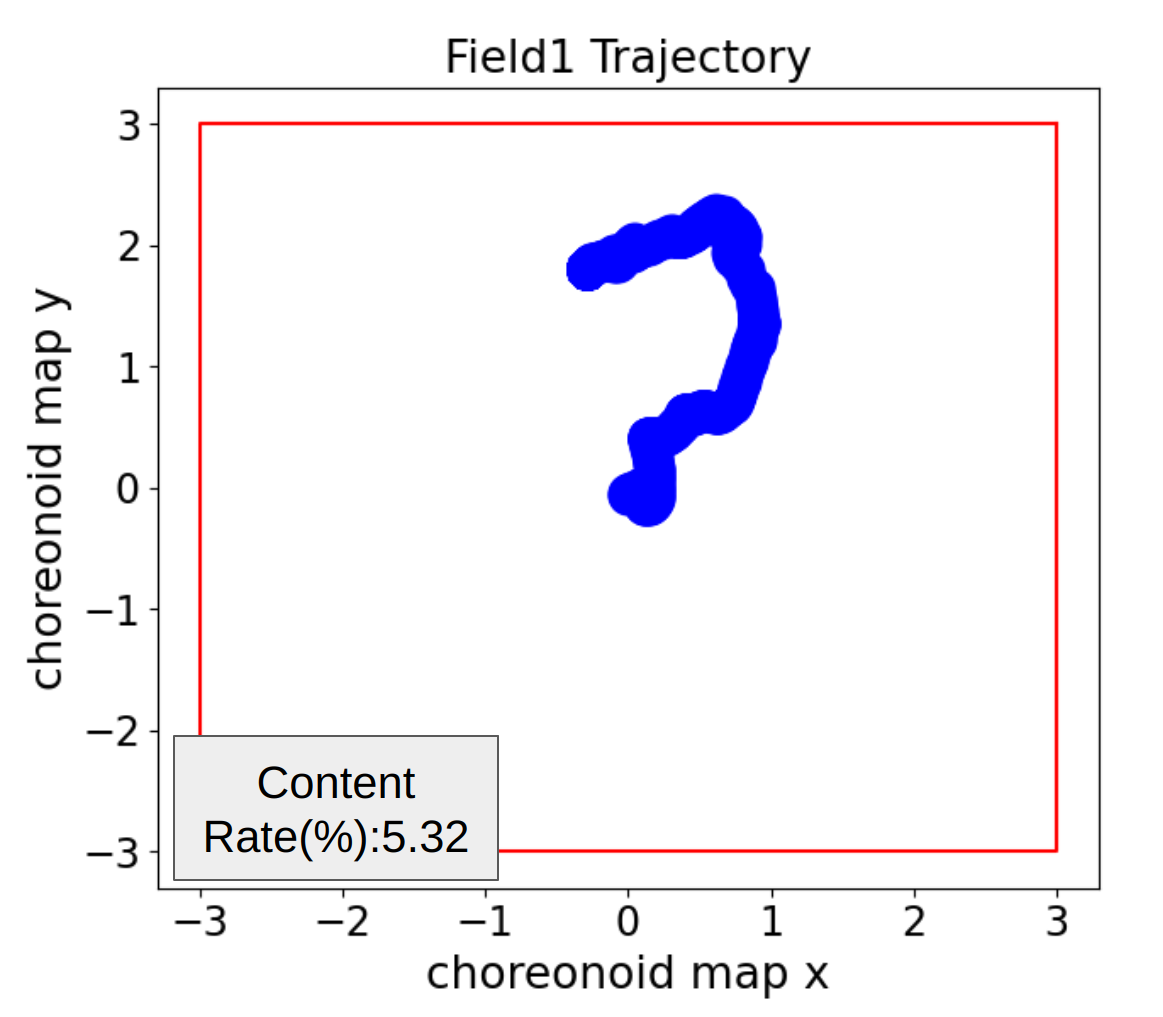
\includegraphics[width=0.6\linewidth]{images/field1_trajectry.png}
   \caption{生成した月面1}
   \label{fig:field1_trajectry}
  \end{center}
 \end{figure}
 \begin{figure}[htbp]
  \begin{center}
   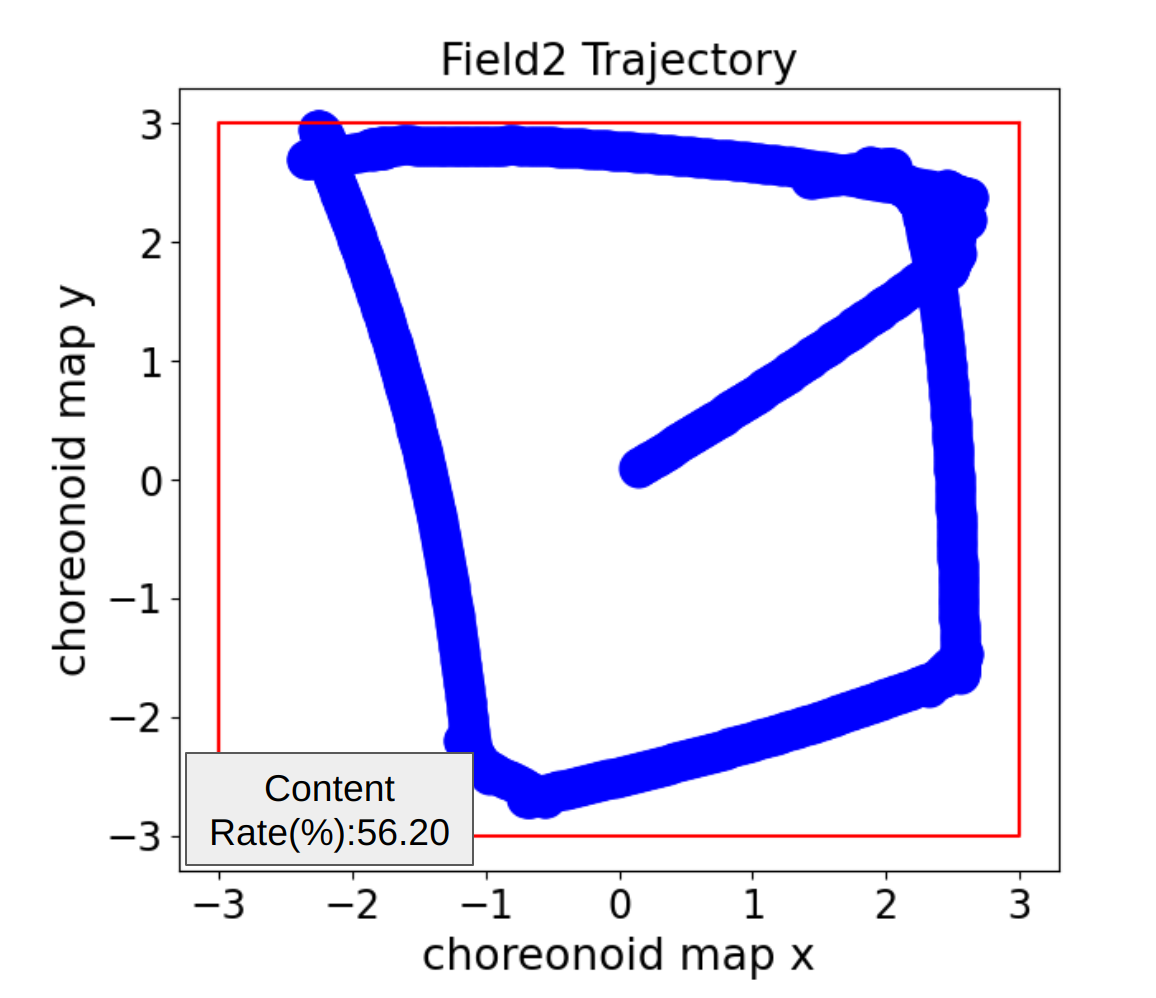
\includegraphics[width=0.6\linewidth]{images/field2_trajectry.png}
   \caption{生成した月面2}
   \label{fig:field2_trajectry}
  \end{center}
 \end{figure}
 \begin{figure}[htbp]
  \begin{center}
   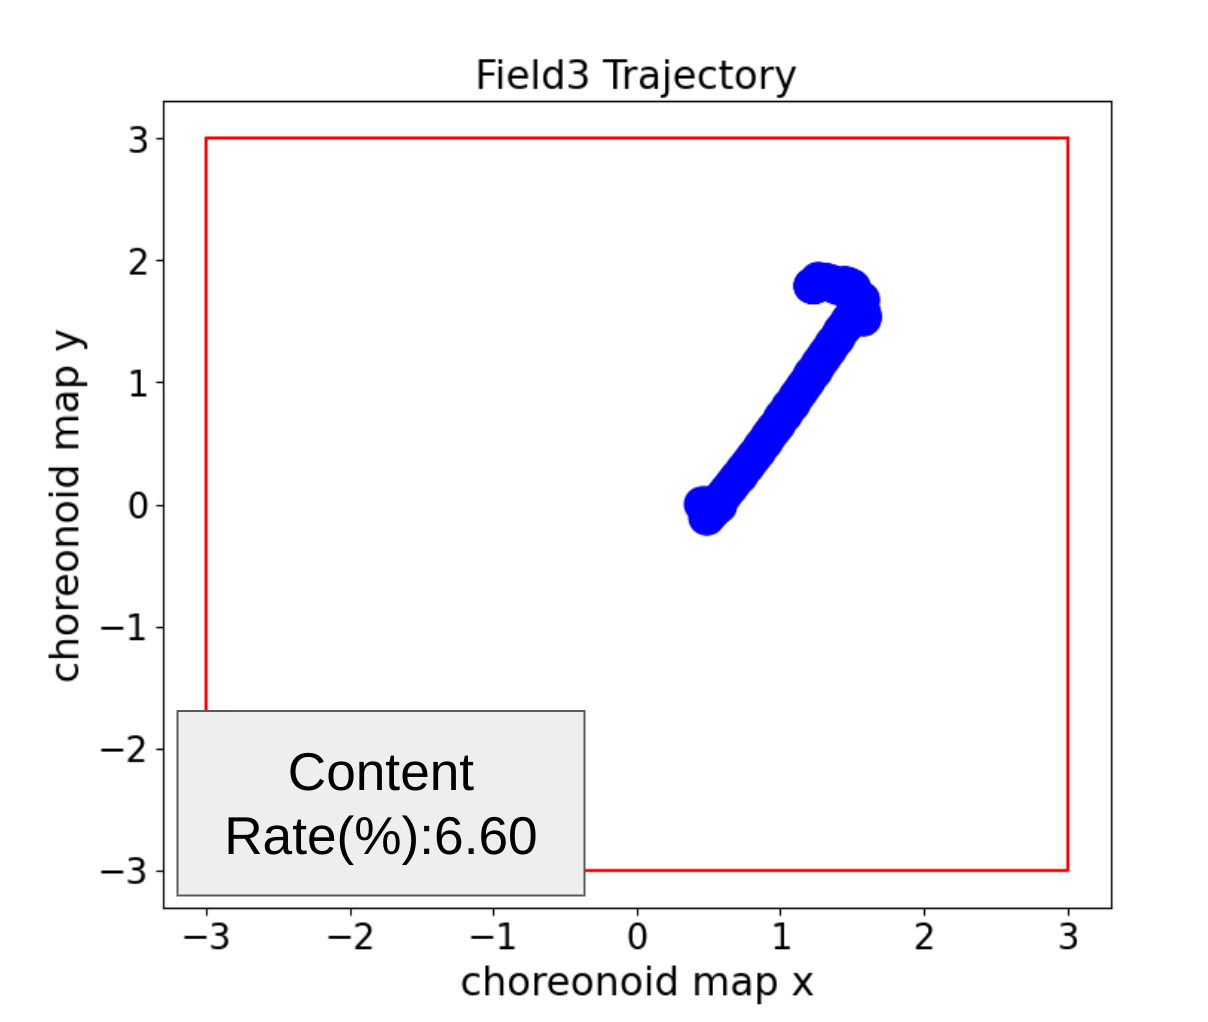
\includegraphics[width=0.6\linewidth]{images/generate_trajectory3.png}
   \caption{生成した月面3}
   \label{fig:generate_trajectory3}
  \end{center}
 \end{figure}
 \begin{figure}[htbp]
  \begin{center}
   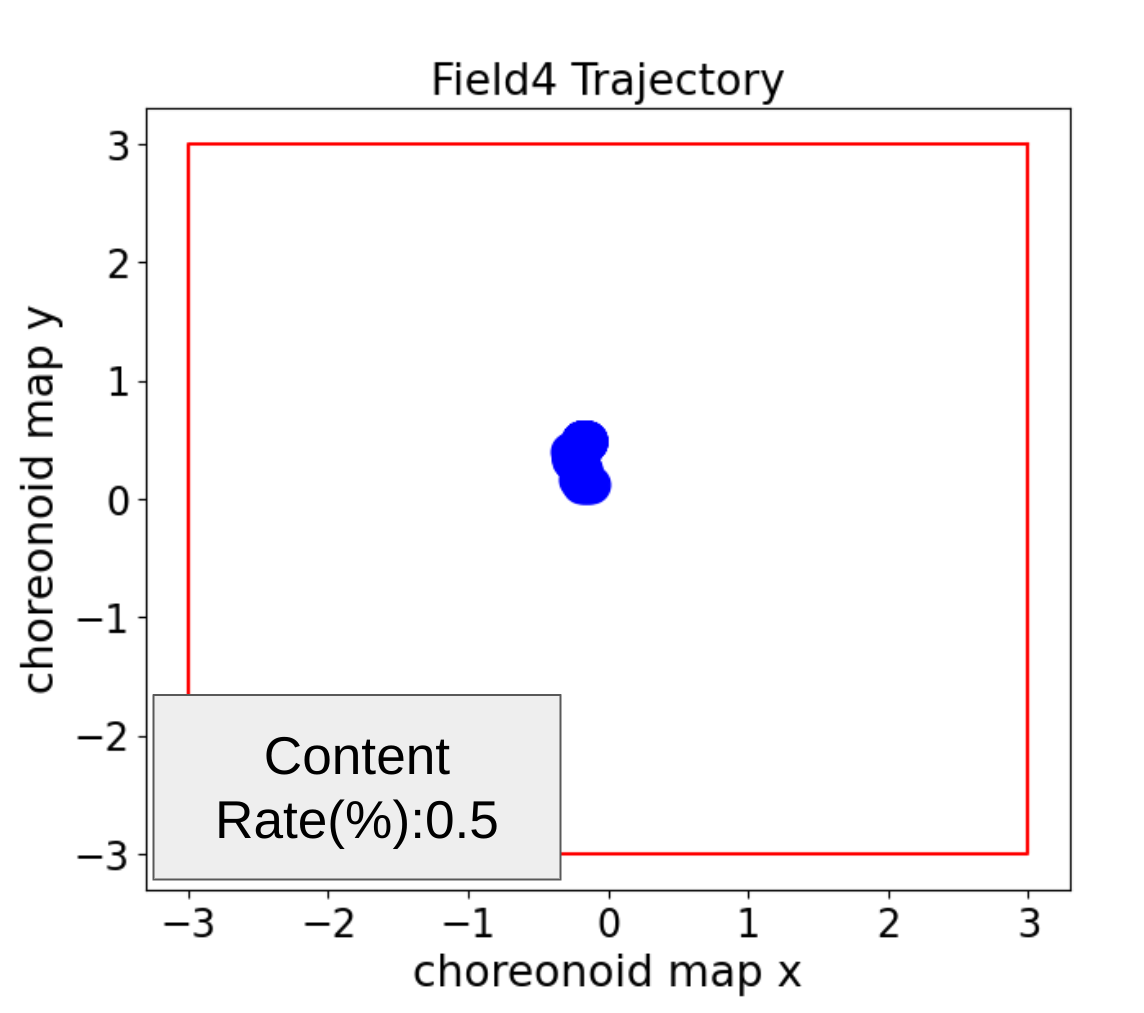
\includegraphics[width=0.6\linewidth]{images/generate_trajectory4.png}
   \caption{生成した月面4}
   \label{fig:generate_trajectory4}
  \end{center}
 \end{figure}

% \begin{figure}[htbp]
%   \begin{minipage}[b]{0.47\linewidth}
%     \centering
%     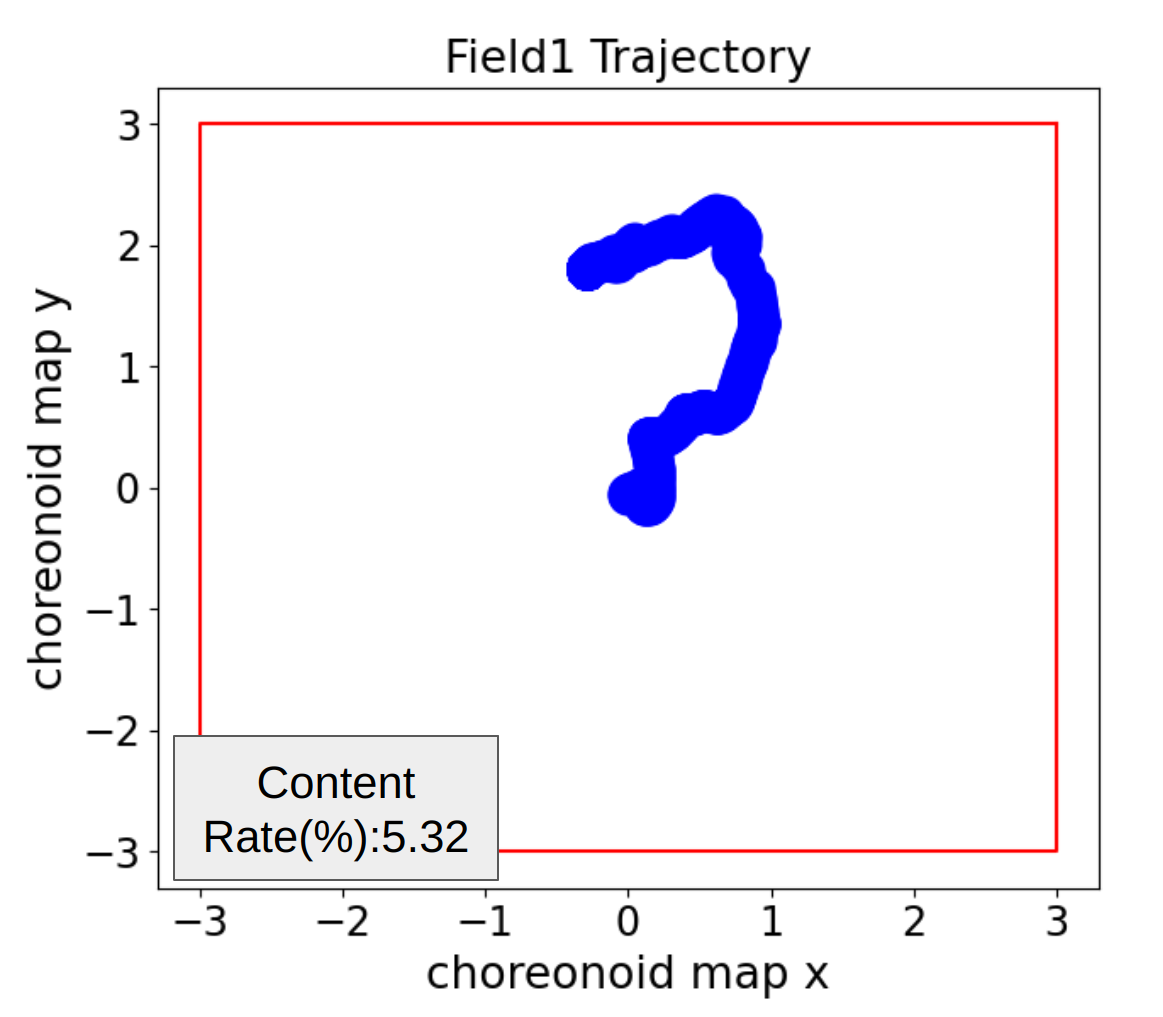
\includegraphics[keepaspectratio, scale=0.178]{images/field1_trajectry.png}
%     \subcaption{生成した月面1}\label{fig:field1_trajectry}
%   \end{minipage}
%   \begin{minipage}[b]{0.47\linewidth}
%     \centering
%     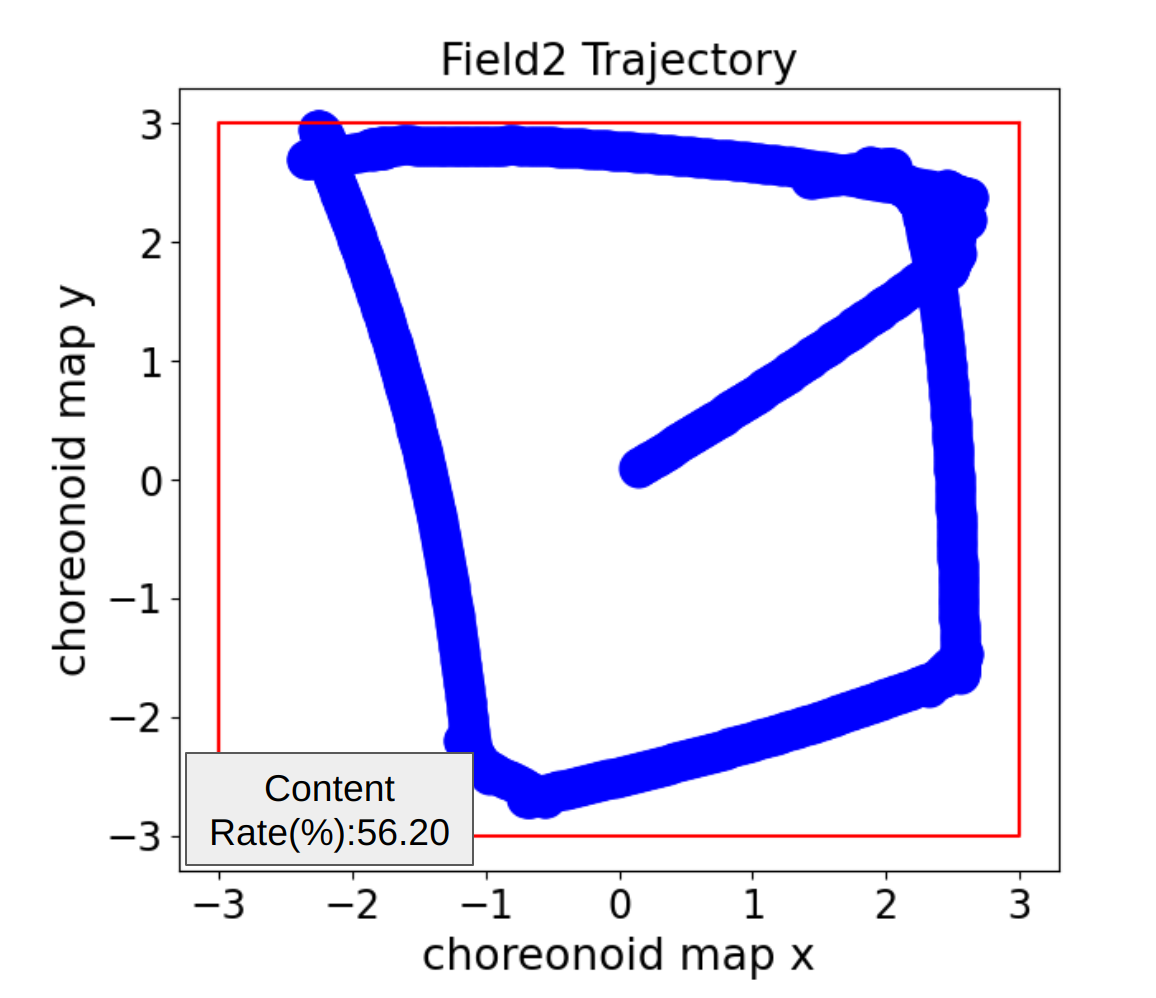
\includegraphics[keepaspectratio, scale=0.183]{images/field2_trajectry.png}
%     \subcaption{生成した月面2}\label{fig:field2_trajectry}
%   \end{minipage}
%   \begin{minipage}[b]{0.47\linewidth}
%     \centering
%     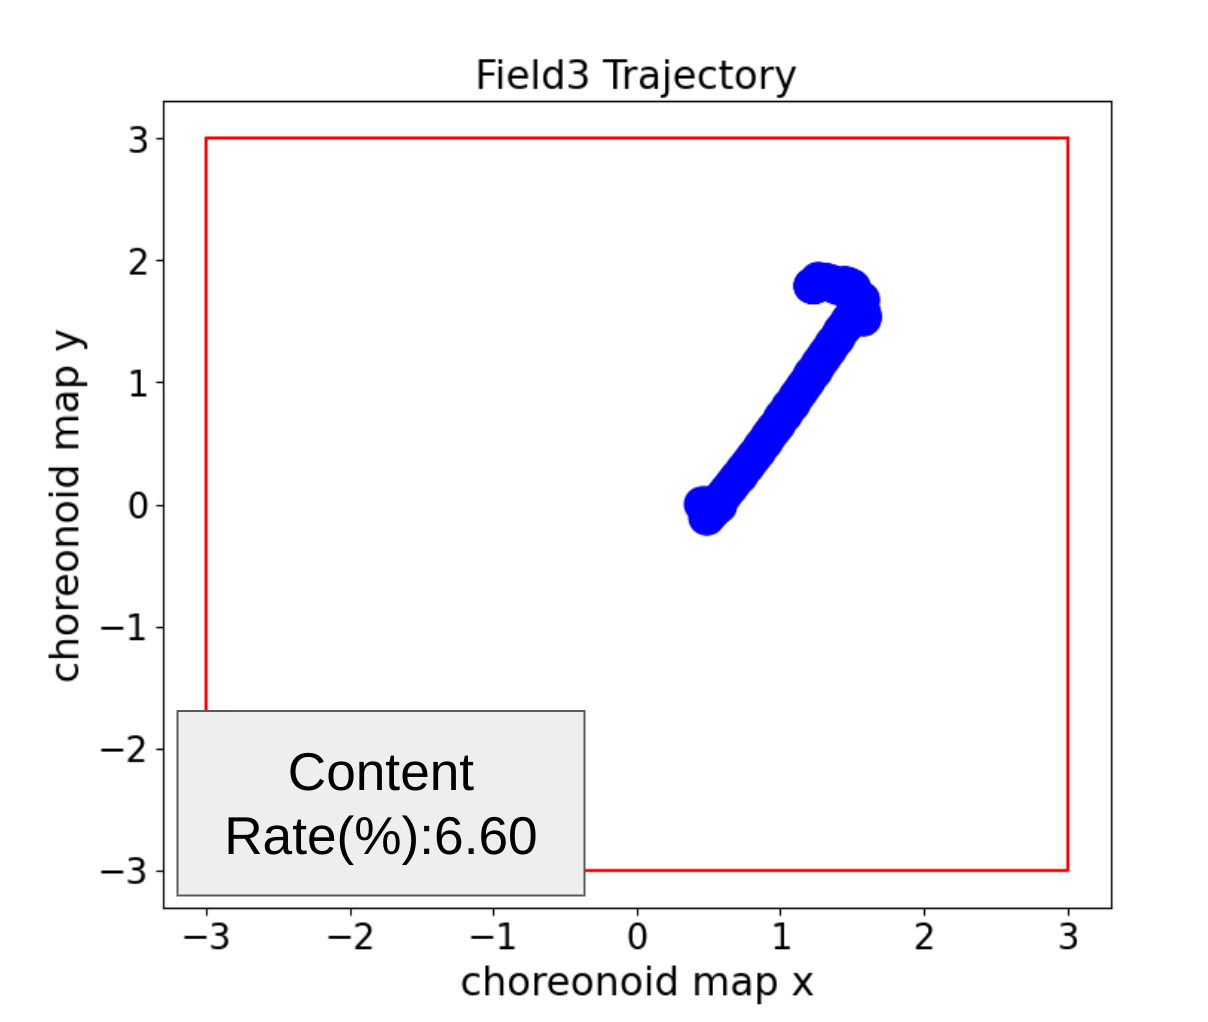
\includegraphics[keepaspectratio, scale=0.178]{images/generate_trajectory3.png}
%     \subcaption{生成した月面3}\label{fig:generate_trajectory3}
%   \end{minipage}
%   \begin{minipage}[b]{0.47\linewidth}
%     \centering
%     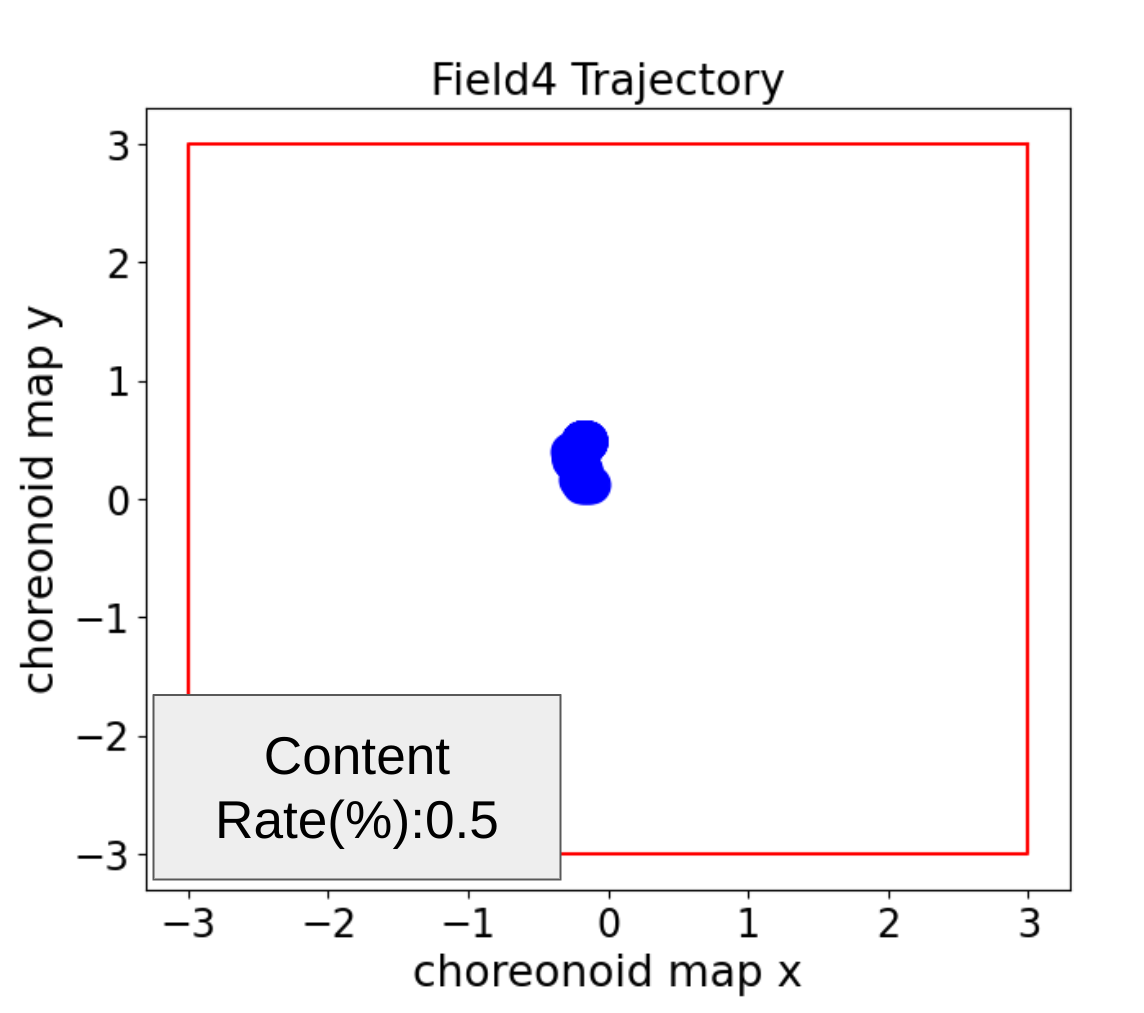
\includegraphics[keepaspectratio, scale=0.183]{images/generate_trajectory4.png}
%     \subcaption{生成した月面4}\label{fig:generate_trajectory4}
%   \end{minipage}
%   \caption{走行した軌跡の結果}\label{fig:results}
% \end{figure}